\documentclass[12pt]{memoir}

\usepackage[letterpaper,left=3.0cm,right=2.5cm,top=3.0cm,bottom=3.0cm]{geometry}

% Style packages
\usepackage[utf8]{inputenc}
\usepackage{graphicx}
\usepackage{lmodern}
\usepackage{xcolor}
\usepackage{xspace}
\usepackage{amsmath}
\usepackage{mathtools}

% Physics packages
\usepackage{braket}
\usepackage{simplewick}

\usepackage{hyperref}
\usepackage[sort&compress]{natbib}

% For license
\usepackage[
    type={CC},
    modifier={by},
    version={4.0},
]{doclicense}

\setsecnumdepth{subsubsection}
\maxtocdepth{subsection}

% Parskip-style
% \setlength{\parindent}{0pt}
\nonzeroparskip


% TODO
\newcommand{\XXX}[1]{\textcolor{red}{#1}}

% Text shortcuts
\newcommand{\mscheme}{\texorpdfstring{$m$-scheme}{m-scheme}\xspace}
\newcommand{\abinitio}{\textit{ab initio}\xspace}

% Units
\newcommand{\mev}{\, \text{MeV}}
\newcommand{\invfm}{\, \text{fm}^{-1}}

% Second quant
\newcommand{\crea}[1]{\ensuremath{a_{#1}^{\dagger}}}
\newcommand{\annih}[1]{\ensuremath{a_{#1}}}
\newcommand{\qpcrea}[1]{\ensuremath{b_{#1}^{\dagger}}}
\newcommand{\qpannih}[1]{\ensuremath{b_{#1}}}

% Commutators
\newcommand{\comm}[2]{\ensuremath{[#1, #2]}}
\newcommand{\anticomm}[2]{\ensuremath{\{#1, #2\}}}

% A-body operators
\newcommand*{\zerobodyop}[1]{\ensuremath{{#1}^{(0)}}}
\newcommand*{\onebodyop}[1]{\ensuremath{{#1}^{(1)}}}
\newcommand*{\twobodyop}[1]{\ensuremath{{#1}^{(2)}}}
\newcommand*{\threebodyop}[1]{\ensuremath{{#1}^{(3)}}}
\newcommand*{\abodyop}[1]{\ensuremath{{#1}^{(A)}}}

% Normal ordering
\newcommand{\nogen}[1]{\ensuremath{\text{N}\left[#1\right]}}
\newcommand{\novac}[1]{\ensuremath{\text{N}_{0}\left[#1\right]}}
\newcommand{\noref}[1]{\ensuremath{\text{N}_{\Phi}\left[#1\right]}}

% Normal ordered operators
\newcommand*{\hnozero}{\zerobodyop{\bar{H}}}
\newcommand*{\hnoone}{\onebodyop{\bar{H}}}
\newcommand*{\hnotwo}{\twobodyop{\bar{H}}}
\newcommand*{\hnothree}{\threebodyop{\bar{H}}}


% Ref state
\newcommand{\refgnd}{\ensuremath{\ket{\Phi}}}
\newcommand{\refhp}[2]{\ensuremath{\ket{\Phi_{#1}^{#2}}}}

% IM_SRG generators
\newcommand*{\genone}{\eta^{(1)}}
\newcommand*{\gentwo}{\eta^{(2)}}
\newcommand*{\genthree}{\eta^{(3)}}

% m-scheme basis
\newcommand*{\emax}{e_{\text{max}}}


\title{Precision nuclear structure in the \\ in-medium similarity renormalization group}

\author{Matthias Heinz}

\date{April 14, 2020}

% \DoubleSpacing
\allowdisplaybreaks

\begin{document}

\frontmatter{}

% Title
\maketitle

\cleardoublepage\section*{Erkl\"arung zur Abschlussarbeit gem\"a\ss\ \S\ 22 Abs.\ 7 und \S\ 23 Abs.\ 7 APB TU Darmstadt}

Hiermit versichere ich, Matthias Heinz, das vorliegende Projekt-Proposal gem\"a\ss{} \S\ 22 Abs.\ 7 APB der TU Darmstadt ohne Hilfe Dritter und nur mit den angegebenen Quellen und Hilfsmitteln angefertigt zu haben. Alle Stellen, die Quellen entnommen wurden, sind als solche kenntlich gemacht worden. Diese Arbeit hat in gleicher oder \"ahnlicher Form noch keiner Pr\"ufungsbeh\"orde vorgelegen.

Mir ist bekannt, dass im Falle eines Plagiats (\S\ 38 Abs. 2 APB) ein T\"auschungsversuch vorliegt, der dazu f\"uhrt, dass die Arbeit mit 5,0 bewertet und damit ein Pr\"ufungsversuch verbraucht wird. Abschlussarbeiten d\"urfen nur einmal wiederholt werden.

Bei der abgegebenen Thesis stimmen die schriftliche und die zur Archivierung eingereichte elektronische Fassung gem\"a\ss{} \S\ 23 Abs. 7 APB \"uberein.

\vskip3ex \hrule \vskip3ex

English translation for information purposes only:

\textbf{Thesis statement pursuant to \S\ 22 paragraph 7 and \S\ 23 paragraph 7 of APB TU Darmstadt}

I herewith formally declare that I, Matthias Heinz, have written the submitted thesis proposal independently pursuant to \S\ 22 paragraph 7 of APB TU Darmstadt. I did not use any outside support except for the quoted literature and other sources mentioned in the paper. I clearly marked and separately listed all of the literature and all of the other sources which I employed when producing this academic work, either literally or in content. This thesis has not been handed in or published before in the same or similar form.

I am aware, that in case of an attempt at deception based on plagiarism (\S\ 38 paragraph 2 APB), the thesis would be graded with 5,0 and counted as one failed examination attempt. The thesis may only be repeated once.

In the submitted thesis the written copies and the electronic version for archiving are pursuant to \S\ 23 paragraph 7 of APB identical in content.

\vskip3ex \hrule

    \vskip5ex
      Darmstadt, den 14.~April 2020
    \vskip6ex
    \rule{0.5\textwidth}{0.4pt}

  {\normalsize(Matthias Heinz)}


% Abstract
\cleardoublepage\chapter*{Abstract}

The in-medium similarity renormalization group (IM-SRG)
is an \abinitio{} many-body method used to great success
to model medium-mass nuclear systems.
Its computational cost scales polynomially,
and its formalism is highly flexible,
leading to multiple variants that have been developed to extend its original closed-shell
formulation to open-shell systems.

The current state-of-the-art implementations truncate the IM-SRG equations
at the normal-ordered two-body level,
the first non-trivial order in the expansion.
In this work, we seek to systematically study the effects
of extending this truncation to the normal-ordered three-body level,
the so-called IM-SRG(3).
We present the results of the current implementation
for ${}^4\text{He}$ and the pairing Hamiltonian,
calculations done to validate our implementation against previous calculations.
We also discuss the steps still to be taken to
arrive at an implementation that will allow for a careful study of the effects
of the IM-SRG(3) truncation for nuclear systems.


% Dedication

% Acknowledgements
% \chapter*{Acknowledgements}


% Table of contents
\cleardoublepage\tableofcontents

% List of tables
% \cleardoublepage\listoftables

% List of figures
\cleardoublepage\listoffigures

% Uncomment for acronyms
% use acronym in text with \ac{label} or \acl{label}
% \cleardoublepage\include{proposal/doc/acronyms}

% Can add list of symbols here
% \cleardoublepage\include{proposal/doc/symbols}

\mainmatter{}

\chapter{Introduction}

Nuclear physics aims to understand systems
where the structure and dynamics are dominated by the strong interaction,
one of the four fundamental forces of nature.
The goals of nuclear science are well-described by the overarching open questions
identified by the U.S.~National Academy of Science in \textit{Exploring the Heart of Matter}~\cite{NRC13heartofmatter}:
\begin{enumerate}
  \item How did matter come into being and how does it evolve?
  \item How does subatomic matter organize itself and what phenomena emerge?
  \item Are the fundamental interactions that are basic to the structure of matter fully understood?
  \item How can the knowledge and technological progress provided by nuclear physics best be used to benefit society?
\end{enumerate}
At the heart of this work is the second question,
with the focus of our attention being on the structure of atomic nuclei.

\begin{figure}[t]
  \centering
  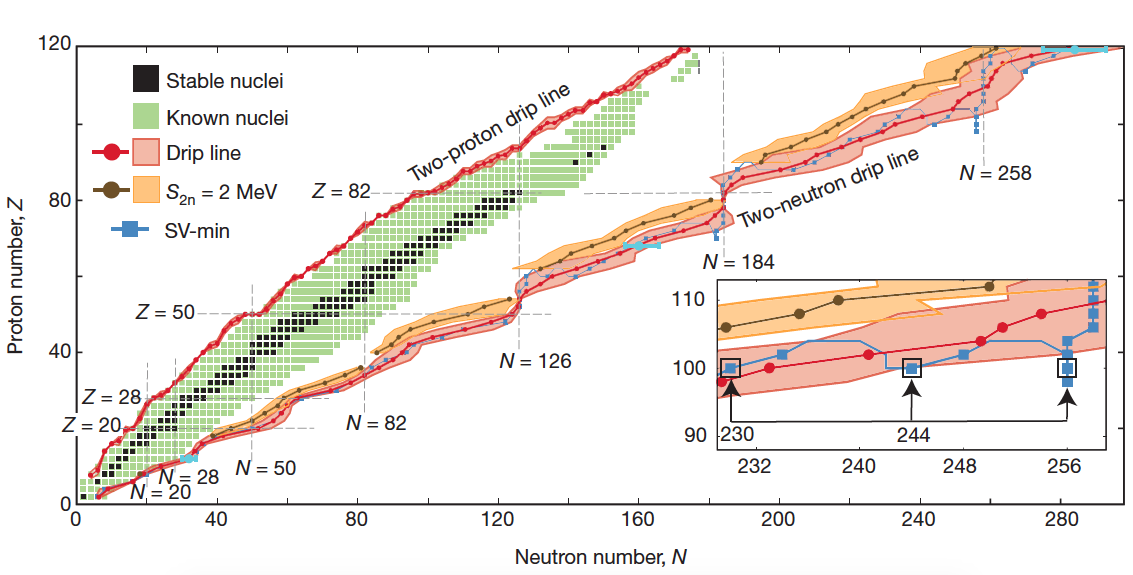
\includegraphics[width=1.0\textwidth]{proposal/doc/images/external/nuclear_landscape.png}
  \caption[
    The nuclear landscape,
    with stable and unstable atomic nuclei denoted by the black and green squares, respectively,
    and a theoretical prediction of the limit of bound nuclei being indicated by the red bands.
  ]{
    The nuclear landscape,
    with stable and unstable atomic nuclei denoted by the black and green squares, respectively,
    and a theoretical prediction of the limit of bound nuclei being indicated by the red bands.
    Figure taken from Ref.~\cite{Erle12limits}.
  }\label{fig:nuclear_landscape}
\end{figure}

Atomic nuclei consist of protons and neutrons, collectively referred to as nucleons.
The interaction between nucleons is dominated by the strong interaction,
and nuclei as self-bound systems of nucleons form as the result of the strong interaction
overcoming a strong kinetic repulsion
due to nucleons being fermions and obeying the Pauli exclusion principle.
Emergent out of the interplay between these two effects,
with contributions from the weak and electromagnetic interactions,
is the nuclear landscape,
shown in Fig.~\ref{fig:nuclear_landscape}.
All of these isotopes arise out of the same basic physics,
with constituent nucleons interacting via basic two- and three-particle interactions.

\textit{Ab initio} nuclear theory aims to realize this understanding of the nuclear landscape
in theoretical calculations,
modeling nuclei from first principles using only the interactions between nucleons as input.
Using only these interactions as inputs means that \abinitio{} methods
have far-reaching predictive power with a large range of applicability.
An additional requirement for \abinitio{} methods is that they are in a theoretical limit exact
and thus systematically improvable for any practical approximation.
This feature also allows the \abinitio{} approach to deliver robust uncertainty estimates,
allowing for the meaningful comparison between experiment and theory
and also between different \abinitio{} theoretical approaches.

\begin{figure}[t]
  \centering
  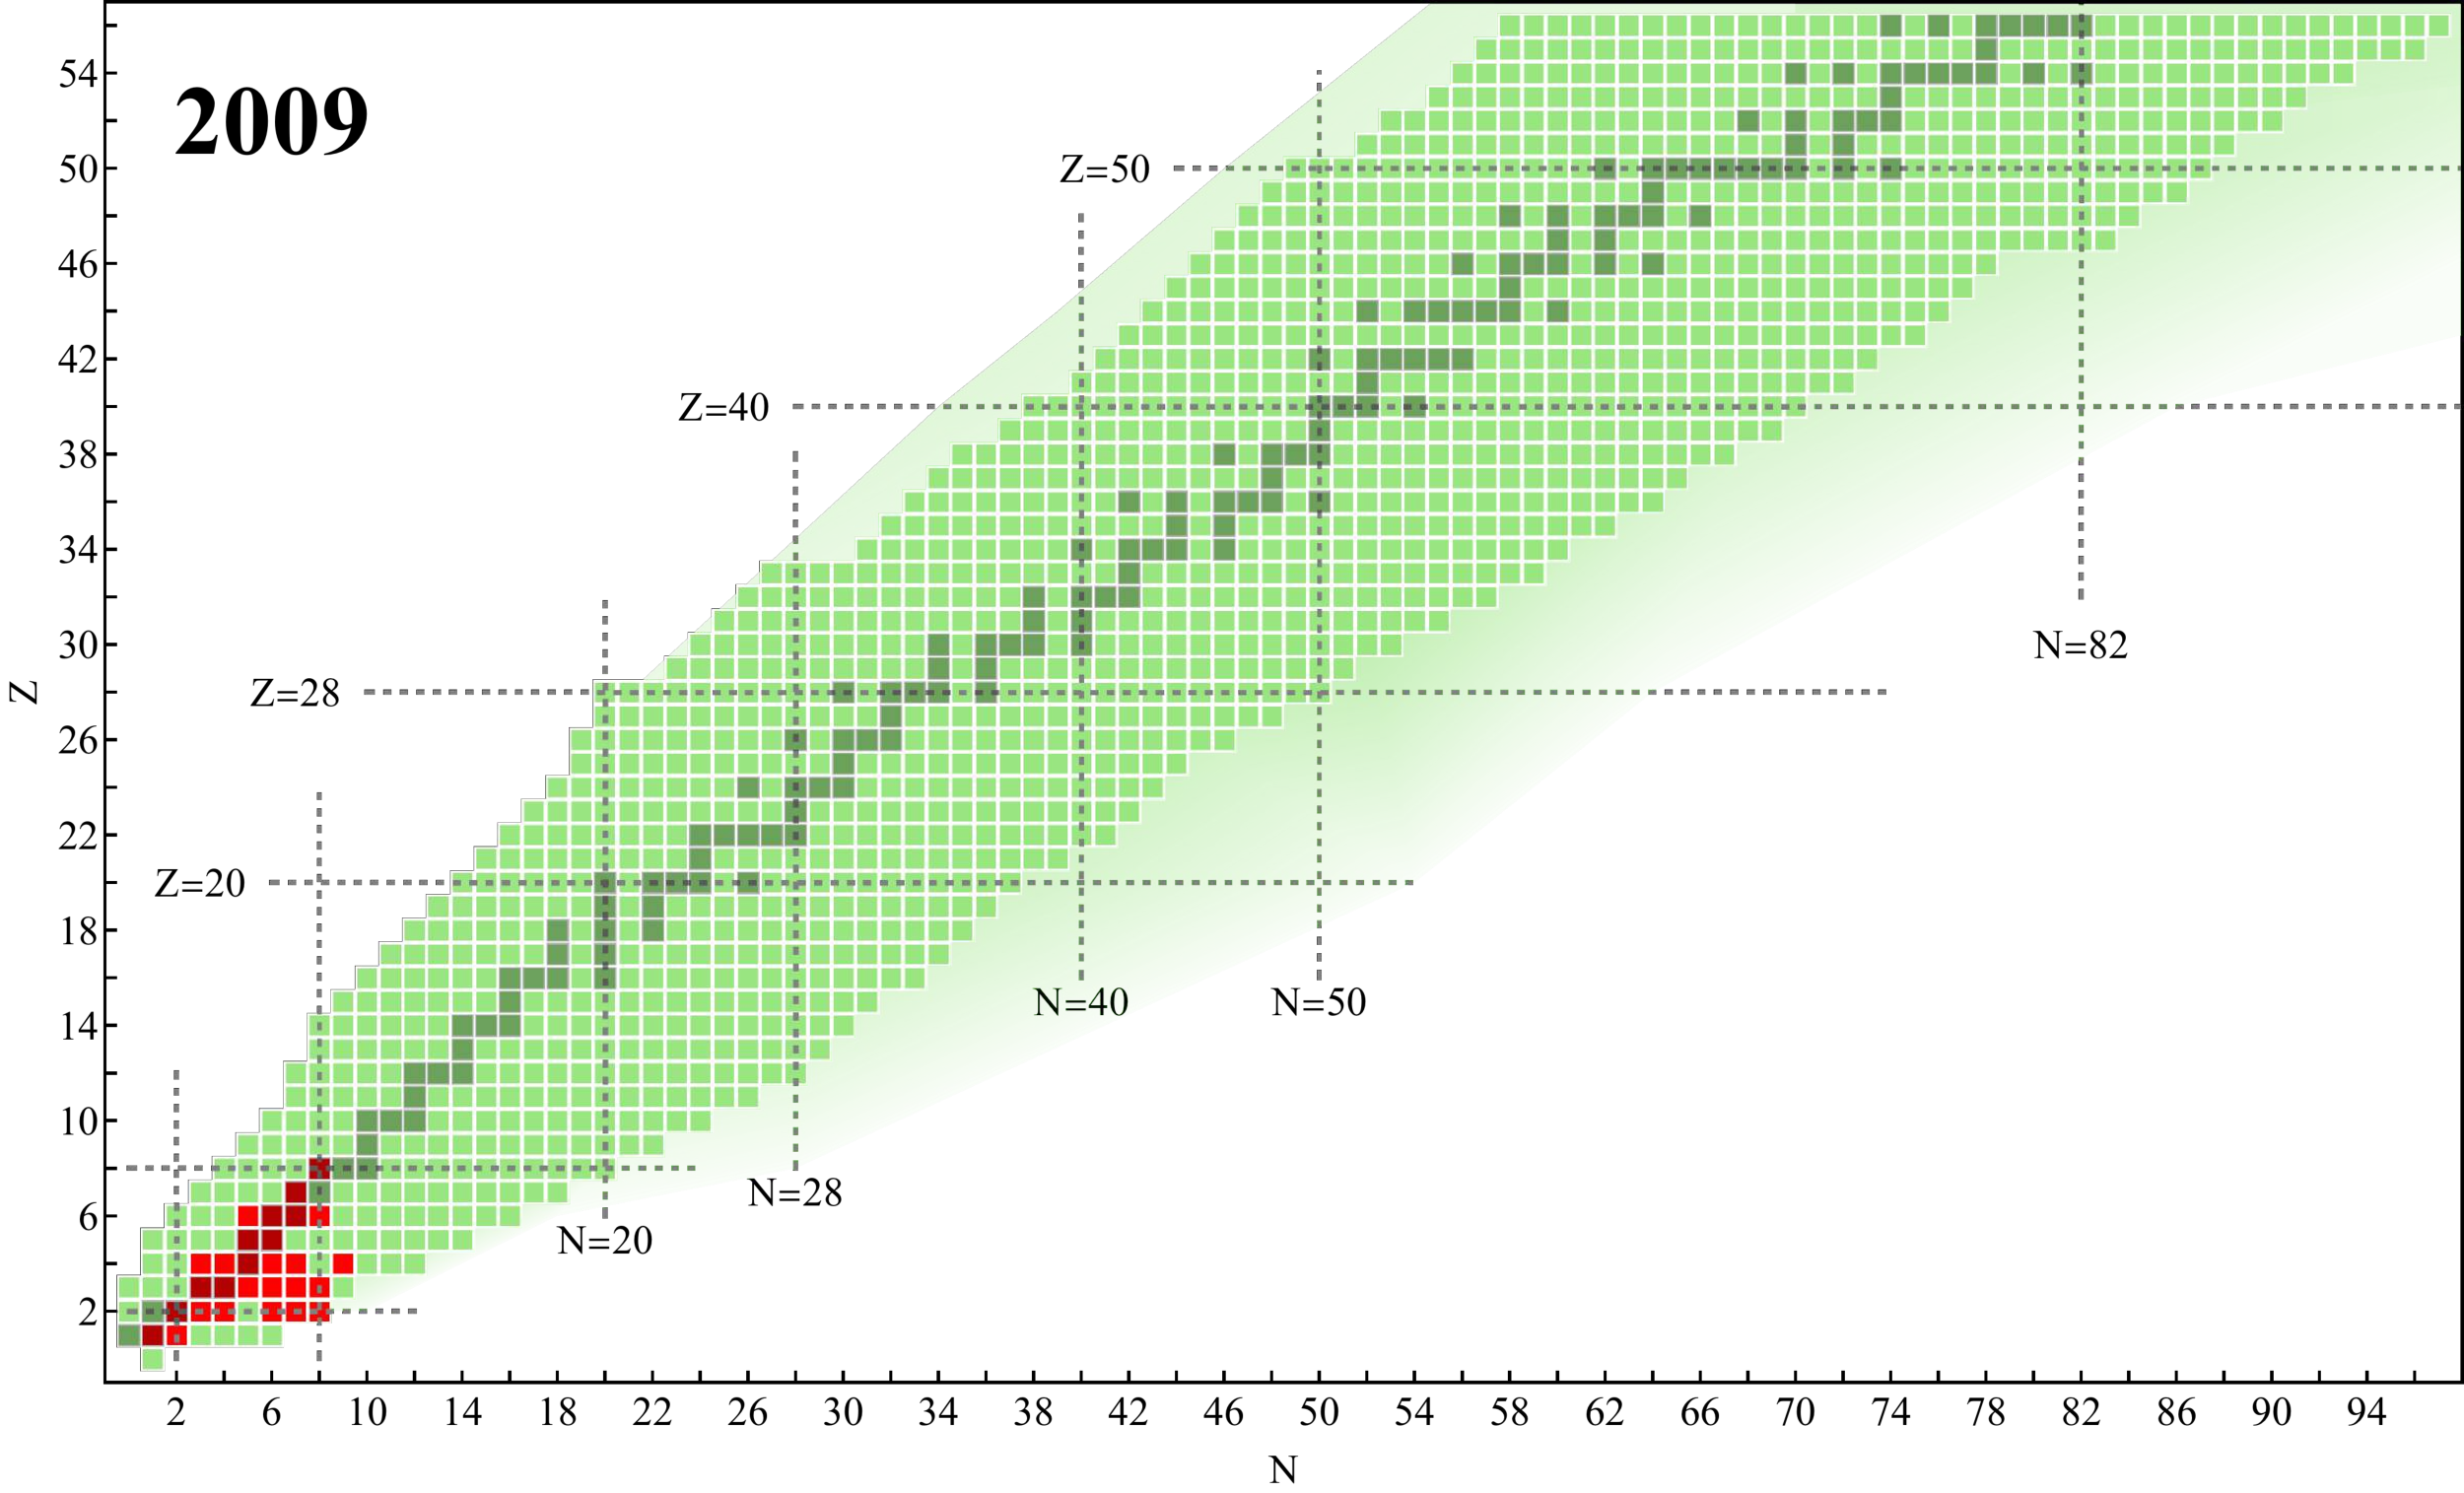
\includegraphics[width=0.45\textwidth]{proposal/doc/images/external/nuclear_chart_2009.pdf}
  \hspace{0cm}
  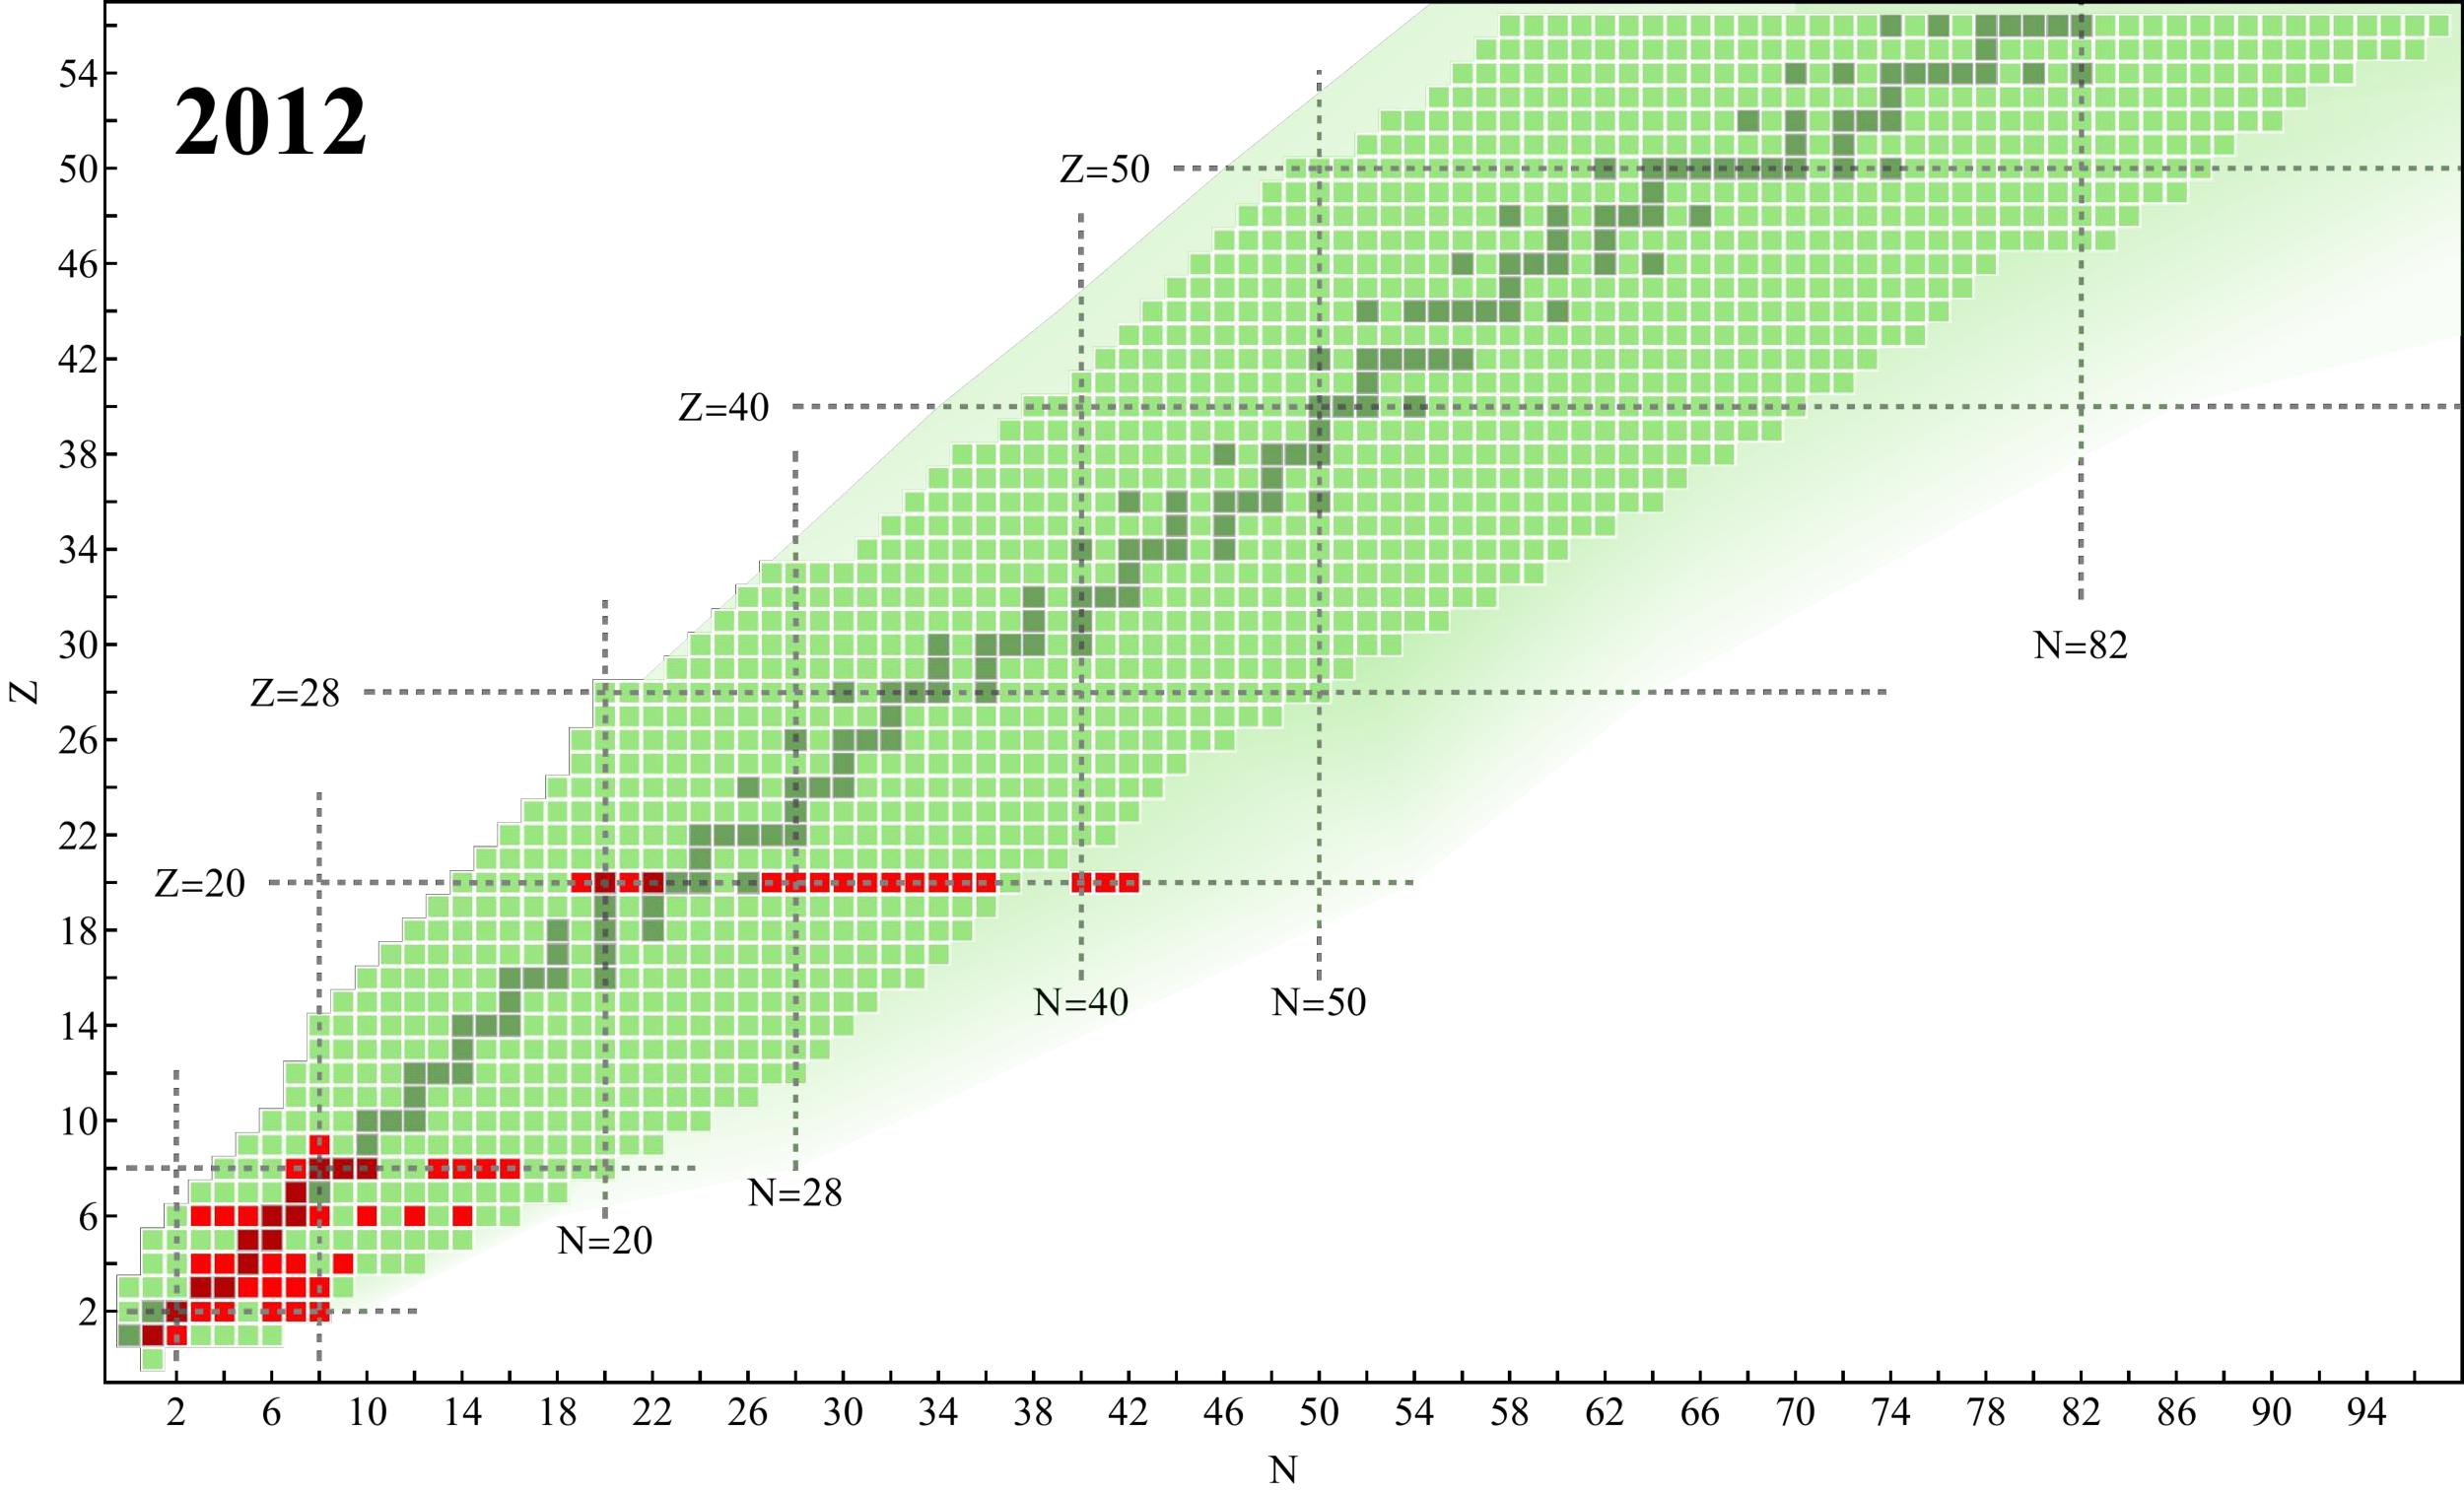
\includegraphics[width=0.45\textwidth]{proposal/doc/images/external/nuclear_chart_2012.pdf}\\
  \vspace{0.05cm}
  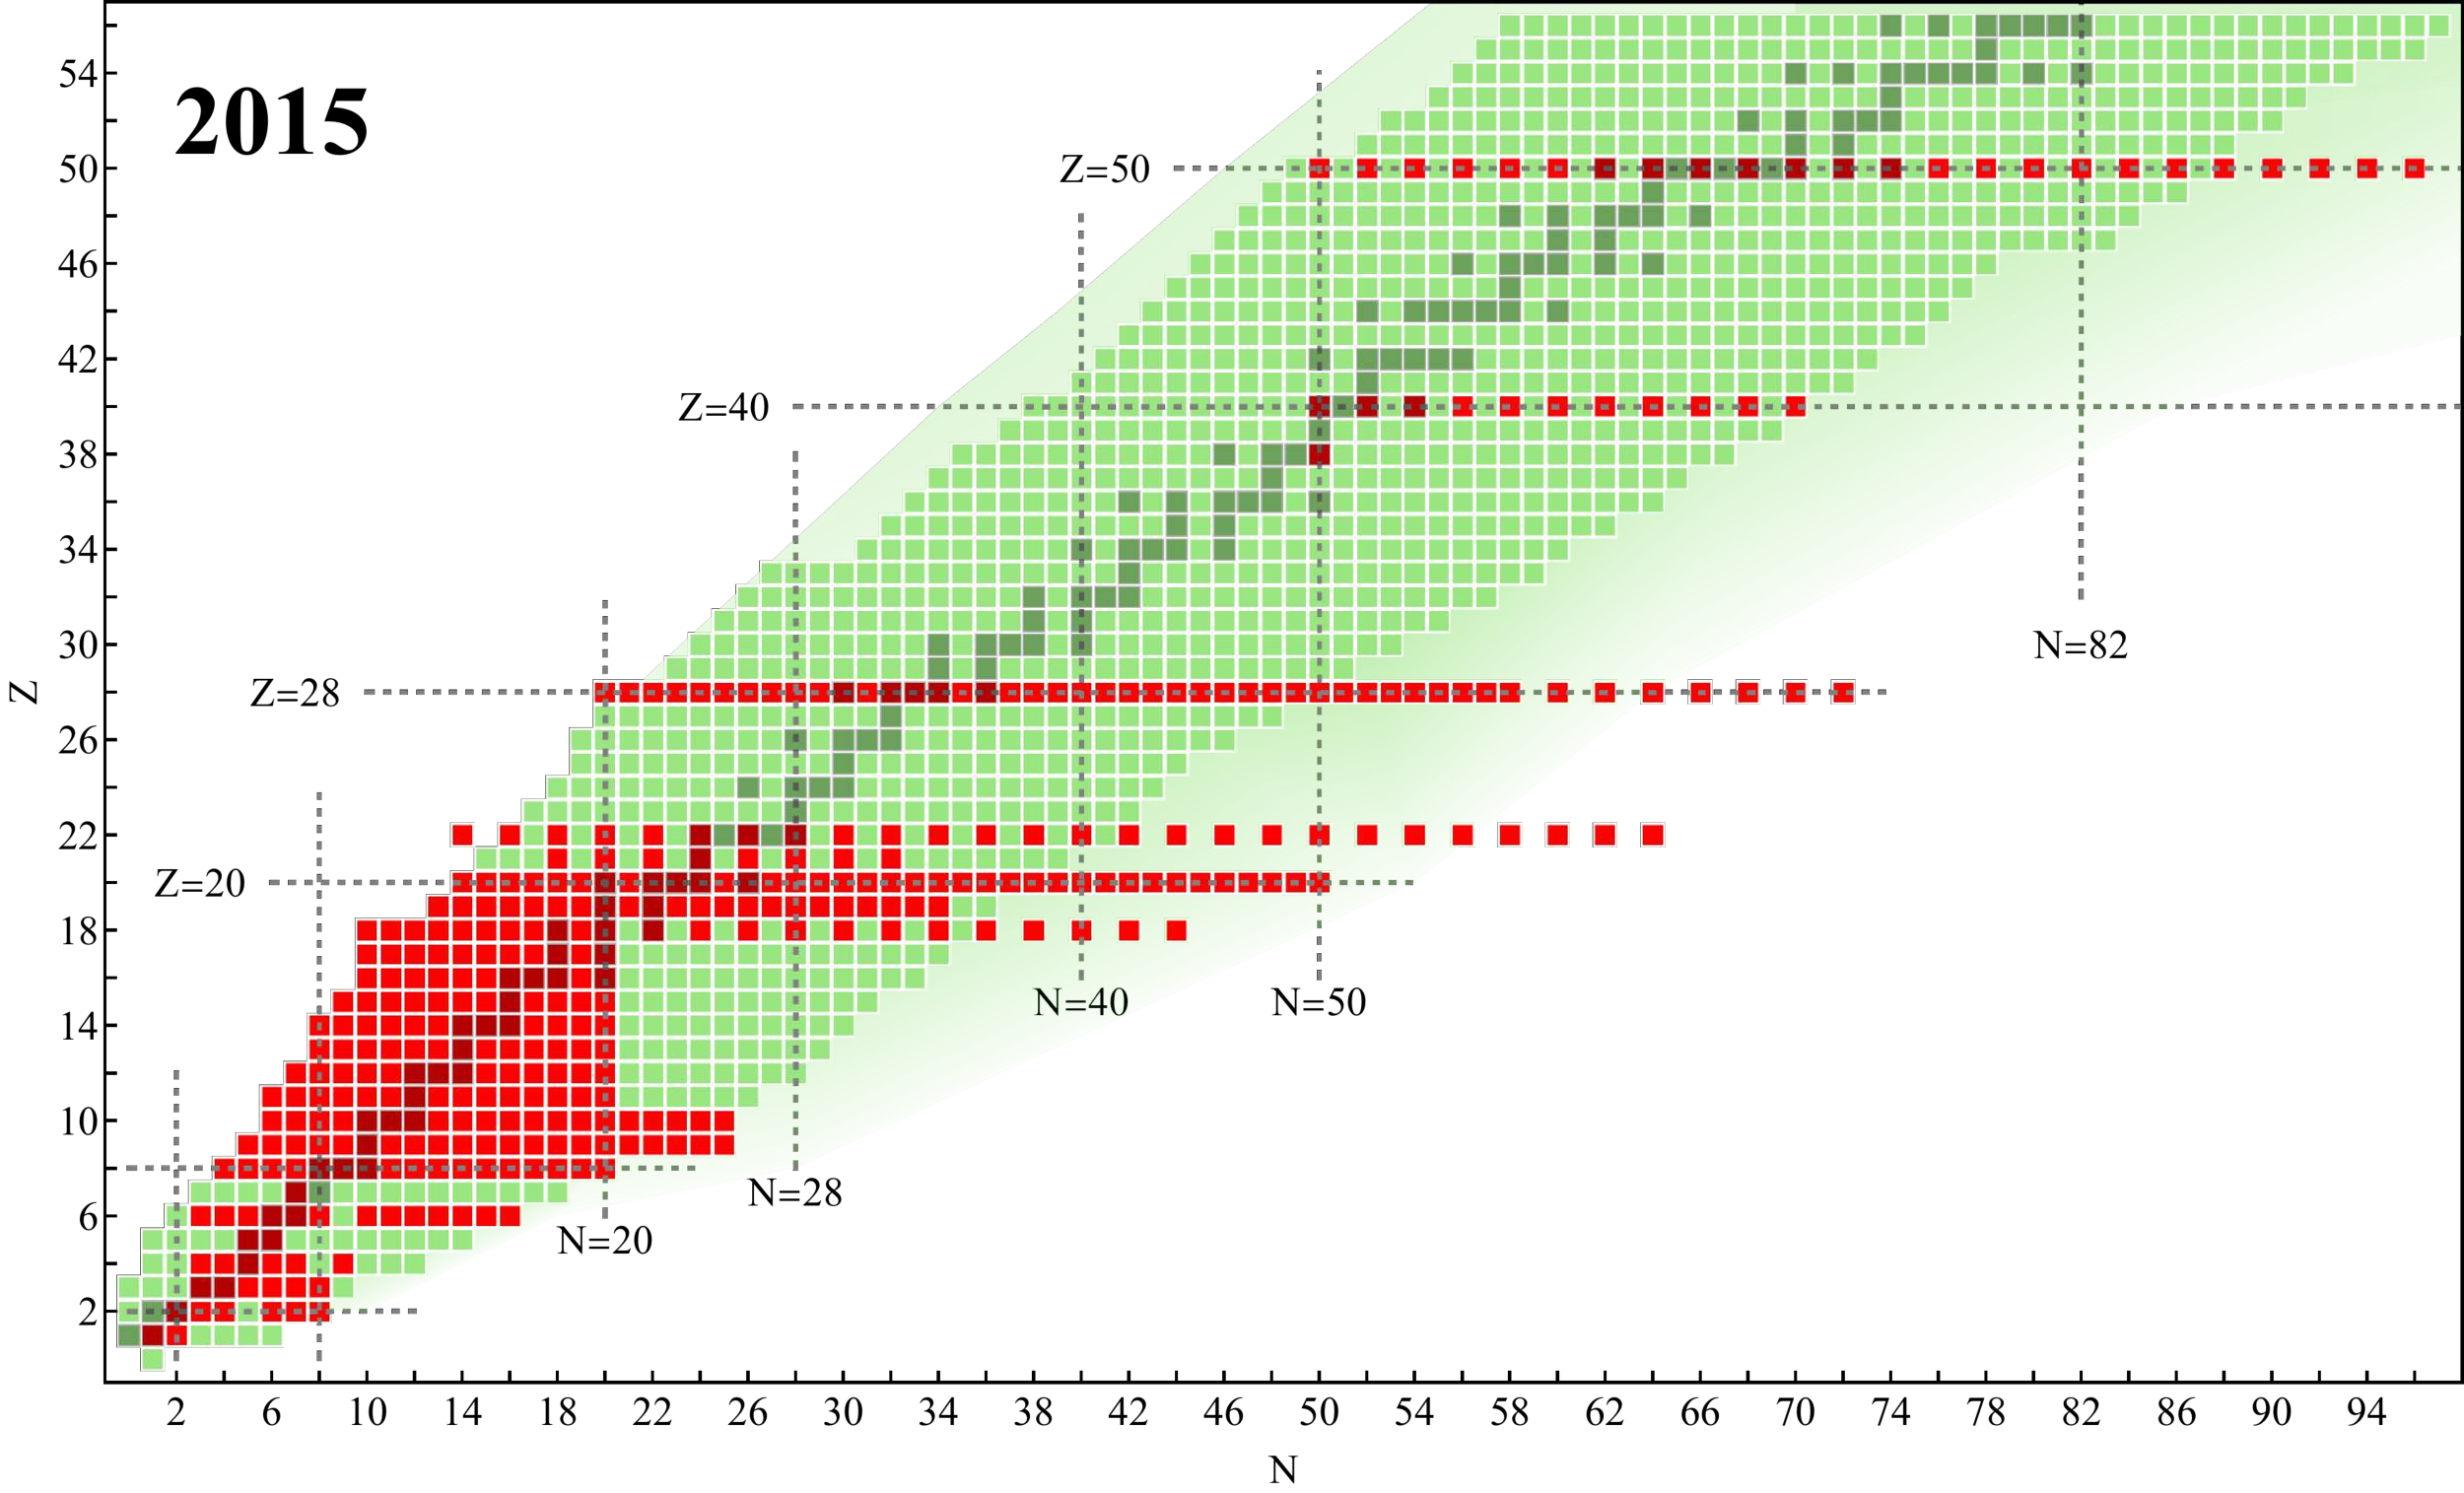
\includegraphics[width=0.45\textwidth]{proposal/doc/images/external/nuclear_chart_2015.pdf}
  \hspace{0cm}
  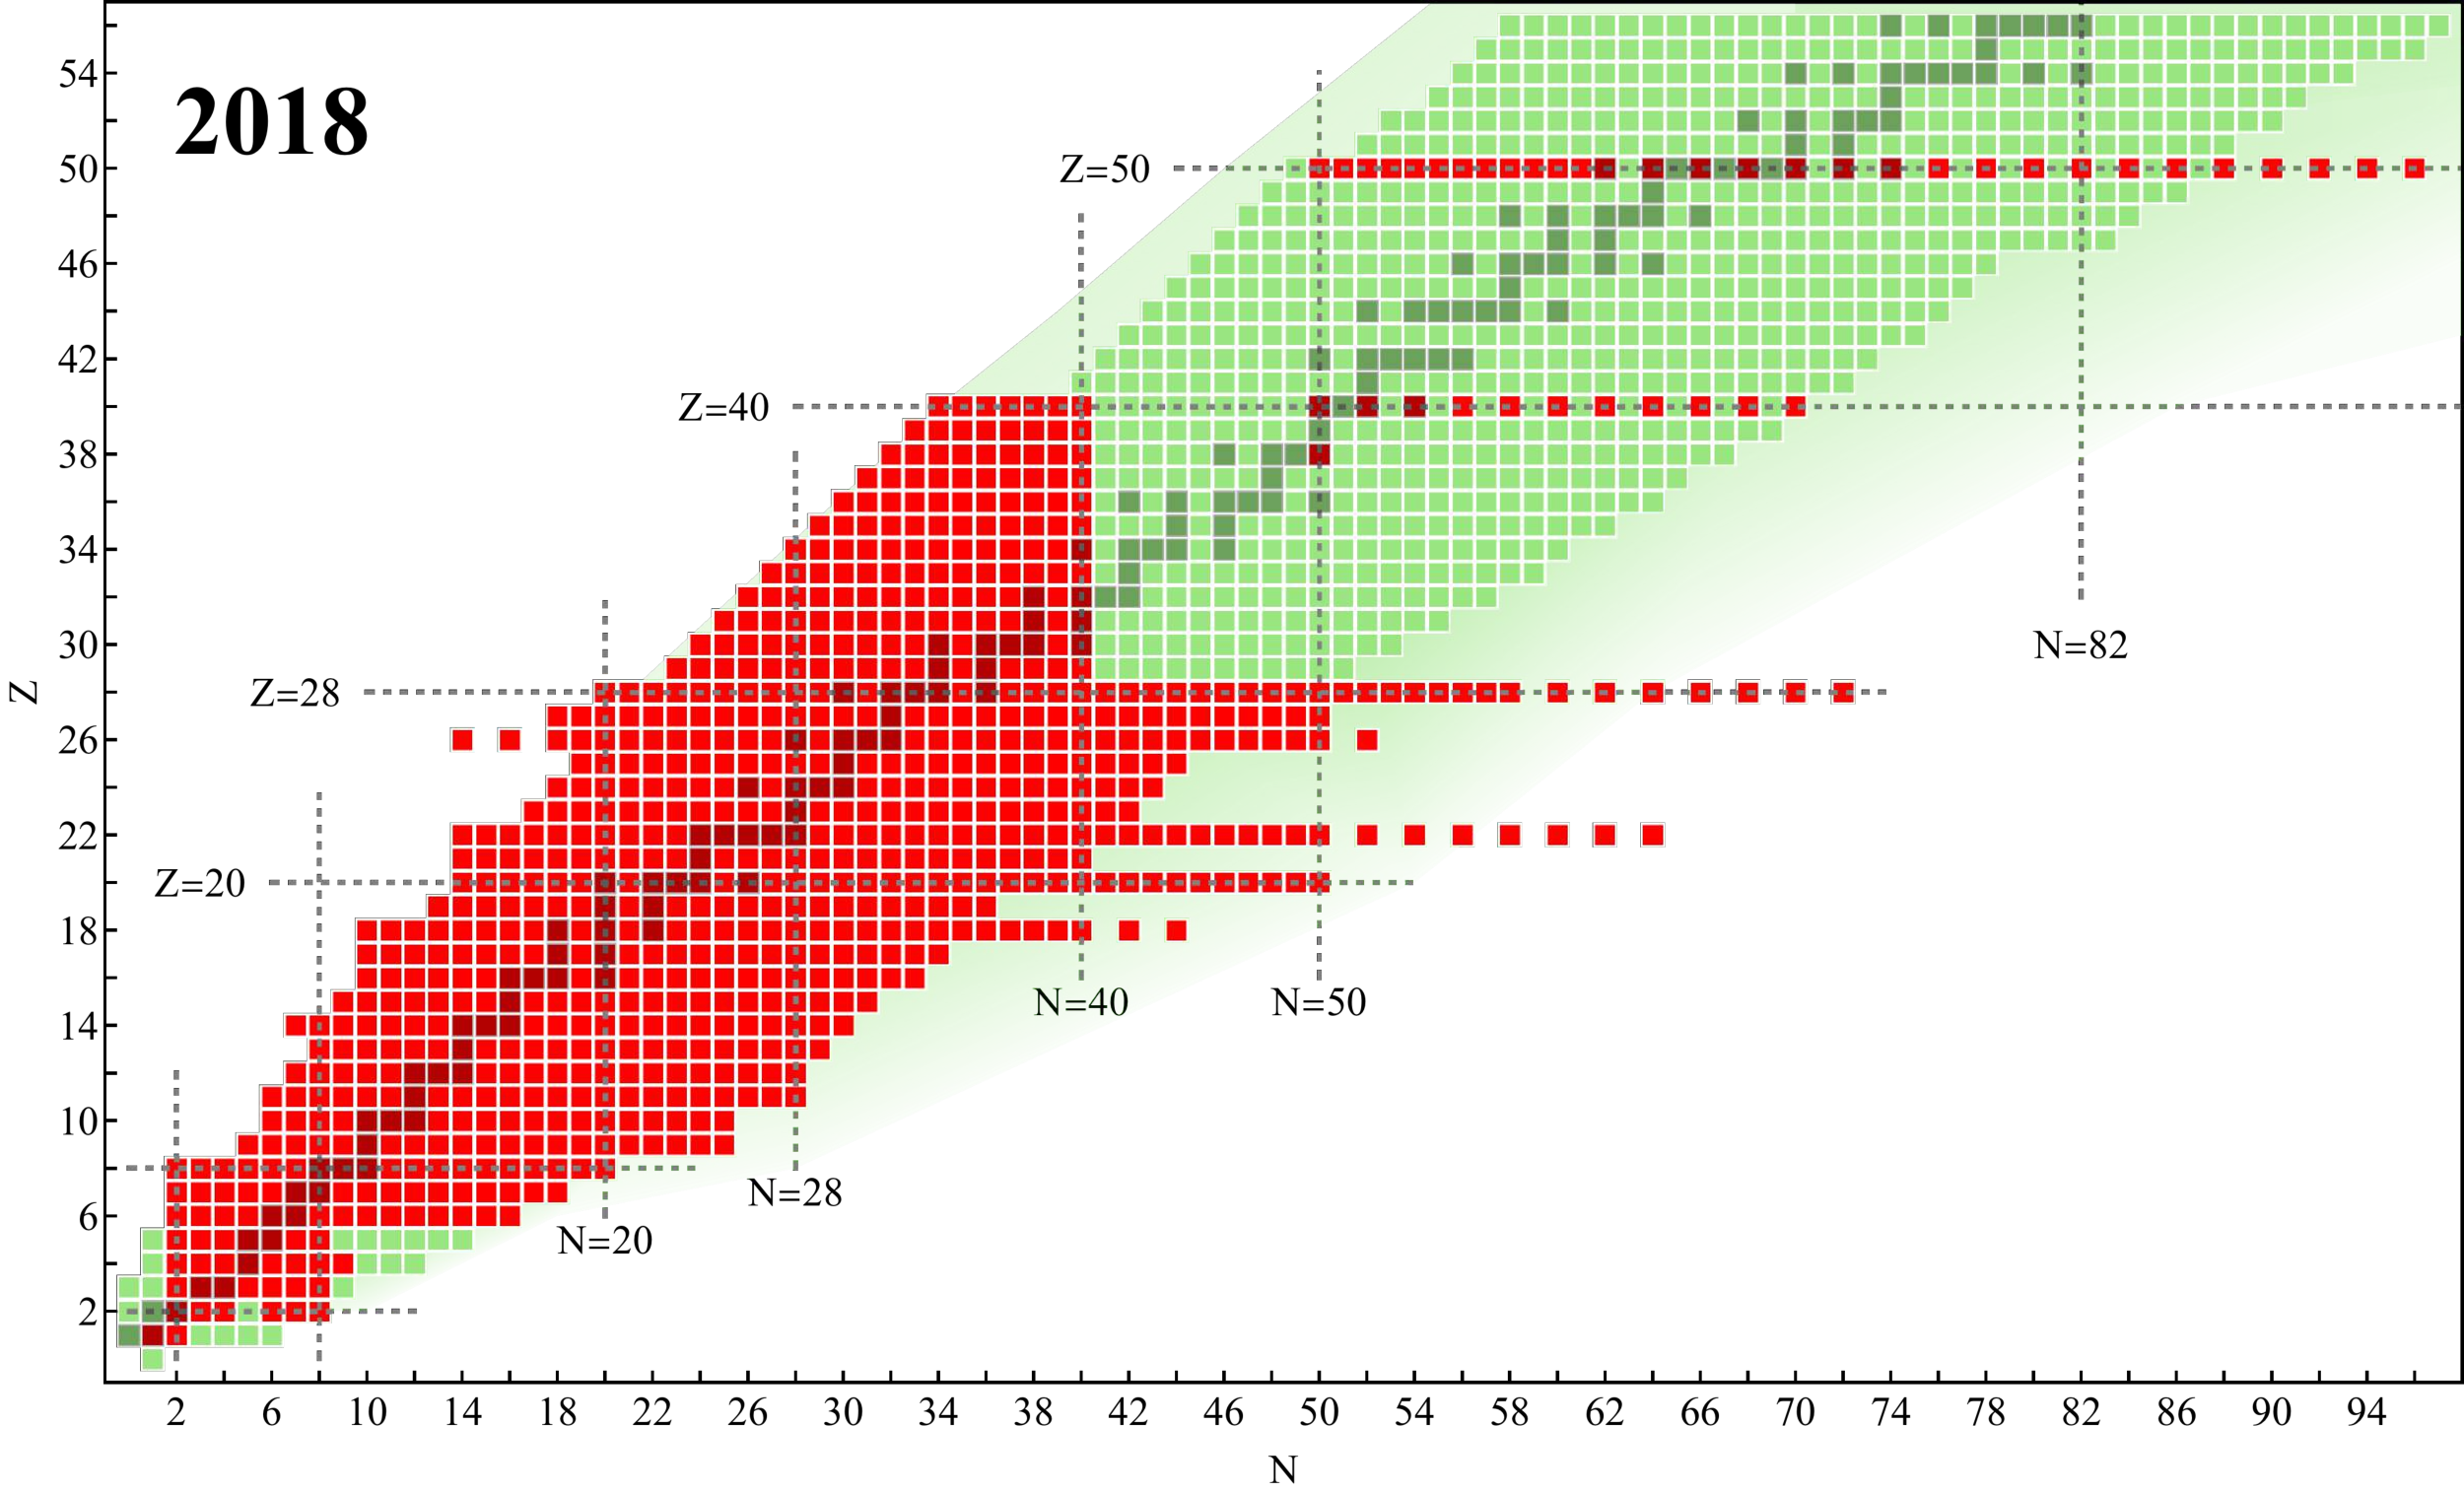
\includegraphics[width=0.45\textwidth]{proposal/doc/images/external/nuclear_chart_2018.pdf}
  \caption[
    Chart of nuclides showing in red nuclei for which \abinitio{} calculations
    involving two- and three-body interactions had been done in 2009 (top left)
    to 2018 (bottom right).
    Only calculations for which covergence with respect to basis size was achieved
    are included in the charts.
  ]{
    Chart of nuclides showing in red nuclei for which \abinitio{} calculations
    involving two- and three-body interactions had been done in 2009 (top left)
    to 2018 (bottom right).
    Only calculations for which covergence with respect to basis size was achieved
    are included in the charts.
    Figure courtesy of Heiko Hergert~\cite{Herg15imsrgphysrep}.
  }\label{fig:ab_initio_conquest}
\end{figure}

Over the past two decades,
the range of \abinitio{} results has expanded rapidly,
as is shown in Fig.~\ref{fig:ab_initio_conquest}.
This change was driven by shift in our understanding of \textit{low-energy}
nuclear physics,
encapsulated in the effective field theory (EFT) and renormalization group (RG) methods.
Underlying both of these ideas is the concept of limited resolution in low-energy physics
and the realization that behavior at short distances (small wavelengths or high energies)
does not affect the big picture at long distances.
Effective field theory methods connect to underlying fundamental theories
explicitly setting the scale to include essential long-distance physics
and generating the most general expansion for the short-distance physics
in terms of contact interactions~\cite{Wein78eft,Hamm19nuceftreview}.
Renormalization group methods allow for varying of the resolution scale,
decoupling or integrating out high-energy details to produce an efficient low-resolution
description of the system at hand~\cite{Wils71rg,Bogn06srg,Bogn09vlowk}.
These two obviously synergistic methods have worked together to produce
low-resolution nuclear forces rooted in the fundamental theory of quantum chromodynamics.

With these new, more efficient low-energy nuclear forces
and the ever increasing available computational resources,
the parallel development of nuclear many-body methods was uncapped.
New developments on old methods, such as coupled cluster,
and the introduction of new methods,
such as the in-medium similarity renormalization group,
have carried \abinitio{} nuclear theory to its present state.

\section{Goals}

The focus of this work will be the in-medium similarity renormalization group (IM-SRG)~\cite{Tsuk10imsrg}.
As indicated by its name,
it brings the RG approach of decoupling low- and high-energy states to the many-body problem,
seeking to decouple the state of a system from its excitations.
It is flexible in that it can target both ground states and low-lying excited states
and calculate energies as well as expectation values for other operators,
and while its original formulation centers on describing closed-shell nuclei,
multiple variants are able to model open-shell nuclei as well.

The current state-of-the-art IM-SRG approaches truncate the formalism at the IM-SRG(2) level,
the first non-trivial truncation where up to normal-ordered two-body operators are kept in the equations.
This truncation has been quite successful,
but for the purposes of reaching higher precision and allowing for quantification
of many-body uncertainties,
extending the truncation to the IM-SRG(3) level is of great interest.
In this work, we aim to systematically study the improvements offered by the IM-SRG(3)
for the ground-state properties of light and medium-mass nuclei.
As a step towards this goal,
we also consider the simpler pairing Hamiltonian system in the IM-SRG.\@

\section{Outline}

The remainder of this thesis is structured as follows:
\begin{itemize}
  \item{In Chapter~\ref{ch:nuclear_forces},
    we introduce some aspects of the theory of nuclear forces.
    We focus on the modern approaches to deriving nuclear forces
    and using choices to improve the convergence of many-body calculations.}
  \item{In Chapter~\ref{ch:many_body},
    we introduce the many-body formalism that underlies the IM-SRG.\@
    We introduce some other many-body methods that also build on this formalism
    to help position the IM-SRG in the greater space of available many-body methods.}
  \item{In Chapter~\ref{ch:imsrg},
    we discuss the IM-SRG in detail.
    We discuss the general formalism and the IM-SRG(2) and IM-SRG(3) truncations.
    We also discuss generator choice,
    which sets how the IM-SRG decouples low and high energies,
    and the Magnus expansion,
    an extension that makes it easier to solve and easier to apply to other observables.}
  \item{In Chapter~\ref{ch:results},
    we discuss the results of our application of our IM-SRG implementation.
    These results are primarily benchmarks to validate the correctness of our implementation.}
  \item{In Chapter~\ref{ch:summary},
    we summarize our results
    and offer an outlook for the next steps towards the goals of this thesis.}
\end{itemize}



\chapter{Nuclear forces}\label{ch:nuclear_forces}

For low-energy nuclear physics,
the goal is to understand the structure and dynamics of systems
with nucleons as constituents.
Thus, a key input into any theoretical calculations of such systems
is the interactions between nucleons.
However, quantum chromodynamics (QCD),
the theory of the strong interaction,
is given in terms of quarks and gluons, not nucleons.
Moreover, at low energies the strong interaction coupling constant $\alpha_s(q^2)$ becomes large,
preventing a fundamental closed-form solution for the interactions between color-neutral hadrons.

As a result, various approaches to determine the interactions between nucleons
have been developed.
One such approach is the phenomenological expansion of the interaction between two nucleons
into terms with different spin, isospin, and angular-momentum dependences.
The (position- and momentum-dependent) strength of each of these terms is then fit to nucleon-nucleon scattering data,
giving rise to, for example, the AV18 potential~\cite{Wiri95AV18}.
This approach has several features that make it undesirable for \abinitio{} nuclear theory.
First, it does not connect to the underlying fundamental theory.
Second, this approach does not prescribe a way to arrive at consistent three-nucleon forces.
Additionally, the fitting procedure often includes scattering data at relatively high energies
when compared to the expected kinetic energy of nucleons in nuclei or nuclear matter,
making such phenomenological interactions highly non-perturbative.

In this chapter, we discuss chiral effective field theory
as an alternative to the phenomenological determination of nuclear forces
and the similarity renormalization group as a method to generally ``soften'' interactions
for many-body calculations.
Then we discuss some details regarding different bases
in which one can represent nuclear potentials.

\section{Nuclear forces from chiral effective field theory}

\begin{figure}[t!]
  \centering
  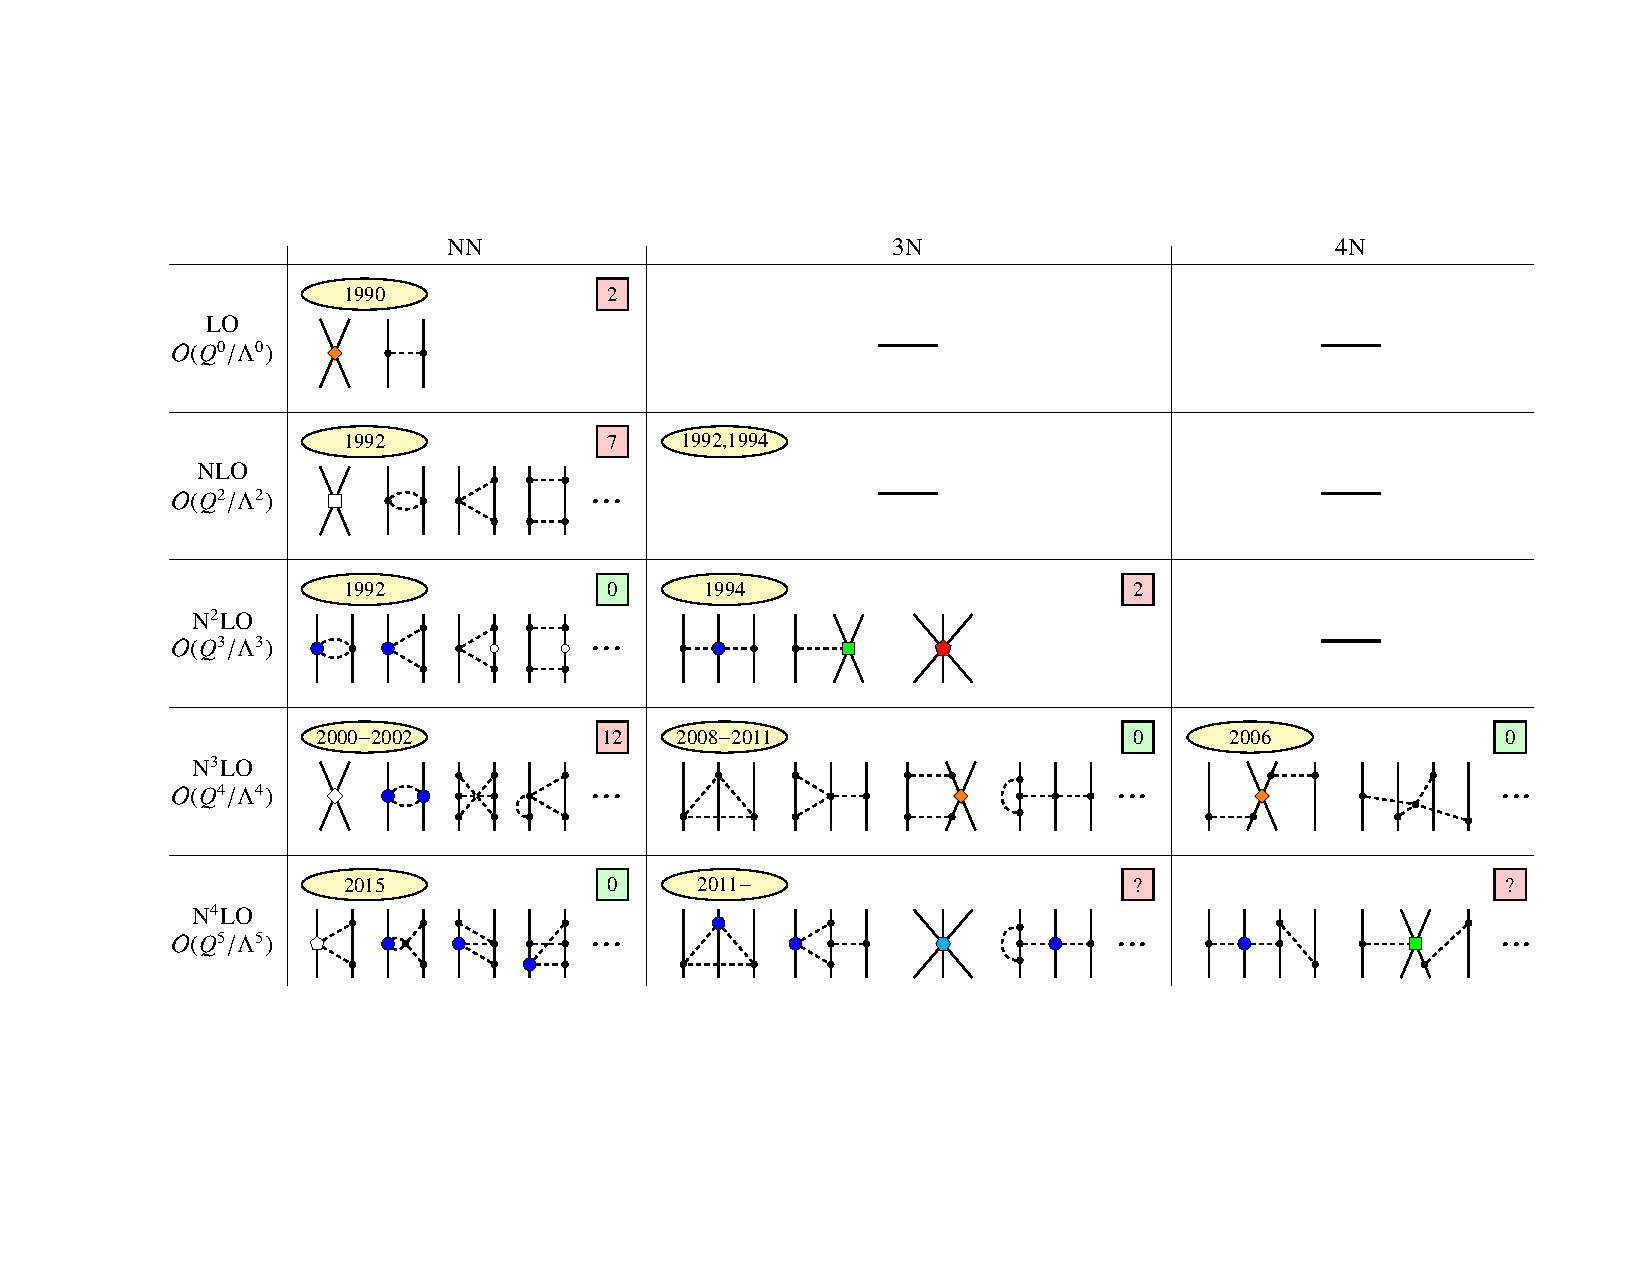
\includegraphics[width=1.0\textwidth]{proposal/doc/images/external/table_norefs.pdf}
  \caption[
    The contributions to NN, 3N, and 4N interactions in chiral EFT
    up to order N4LO.\@
    Solid lines indicate nucleon propagators.
    Dashed lines indicate pion propagators.
    The number of new LECs for the new interaction contributions at each new order
    is shown in the top right corner.
  ]{
    The contributions to NN, 3N, and 4N interactions in chiral EFT
    up to order N4LO.\@
    Solid lines indicate nucleon propagators.
    Dashed lines indicate pion propagators.
    The number of new LECs for the new interaction contributions at each new order
    is shown in the top right corner.
    Figure taken from Ref.~\cite{Hebe20habi}.
  }\label{fig:chiefttable}
\end{figure}

A modern approach to deriving nuclear potentials is chiral effective field theory.
The EFT approach allows one to systematically construct a field theory that approximates
a more fundamental theory in a low-energy domain~\cite{Epel08chiraleft,Mach11chiraleft,Hamm19nuceftreview}.
In this apppropriately chosen domain,
one can use the most efficient degrees of freedom to formulate the theory.
The construction of the theory relies on knowing the symmetries (exact and approximate) of the underlying theory.
Constructing the most general Lagrangian consistent with these underlying symmetries
yields the most general $S$-matrix~\cite{Wein78eft}.

To construct an effective field theory, one identifies the degrees of freedom one wants to work with
and identifies a high-momentum scale $\Lambda$ of the underlying theory that characterizes physics no longer resolved by the EFT~\cite{Hamm19nuceftreview}.
The EFT then should be an efficient, approximately complete description of the relevant physics
at momenta $Q$ small compared to $\Lambda$.
The chosen degrees of freedom are used to construct the most general Lagrangian consistent with the underlying symmetries,
which will have an infinite number of terms each with their own coefficients,
the so-called low-energy constants (LECs).
The EFT can then be used to calculate observables up to some precision in an expansion in $Q/\Lambda$,
made systematic by a power-counting approach.

For chiral EFT,
the underlying theory is QCD in the light-quark sector
(here this means only up and down quarks),
where the Lagrangian has an approximate chiral symmetry $\text{SU}{(2)}_L \times \text{SU}{(2)}_R$
in the limit of vanishing quark masses and no electroweak interactions~\cite{Hamm19nuceftreview}.
This symmetry is spontaneously broken,
giving rise to the pion as the Goldstone boson associated with the broken $\text{SU}{(2)}_A$ symmetry,
as well as explicitly broken by the non-zero quark masses~\cite{Page74chisymm}.
A logical choice of degrees of freedom is then nucleons and pions.
The high-momentum scale $\Lambda_b$ is set by the lightest meson not included in our degrees of freedom,
the $\rho$ meson with a mass of $m_{\rho}\approx 770 \mev$~\cite{Mach11chiraleft}.
The low-momentum scale is a collective scale given by $\text{max}(Q, m_{\pi})$.

The resulting potential contributions from chiral EFT have either explicit pion exchanges
or contact interactions with LECs describing short-range physics unresolved by the EFT,
as shown in Fig.~\ref{fig:chiefttable}.
The first consistent three-nucleon (3N) interactions appear at next-to-next-to-leading order (N2LO),
and the first four-nucleon (4N) interactions appear at next-to-next-to-next-to-leading order (N3LO).
Among the features that make EFTs so powerful is that they allow for clear error estimates~\cite{Furn15bayesuq,Epel14ekm1,Epel14ekm2},
given proper power-counting,
by considering the order-by-order convergence of observables
and seeing that the orders left out due to a truncation at order $N$ should contribute something like
\begin{equation}
  \Delta O^{(N)} \sim O {\left(\frac{\text{max}(Q, m_{\pi})}{\Lambda_b} \right)}^{N+1}\,,
\end{equation}
where $O$ is the exact result for some observable of interest
(see Fig.~\ref{fig:chieft_uq}).

For potentials from chiral EFT,
at each order a finite number of undetermined LECs are introduced with the new contributions to the potential.
For nucleon-nucleon (NN) interactions, these can be determined by fitting to \textit{low-energy} scattering data.
For 3N interactions, the relevant LECs must be fit to three-body or four-body observables.
Typical choices for these observables at N2LO, where two three-body LECs, $c_D$ and $c_E$, need to be fit,
are the triton binding energy and either the triton half-life or the ${}^4\text{He}$ charge radius~\cite{Hebe20habi}.
Additionally, some contributions at later orders in the expansion only depend on LECs from previous orders.
For example, the 3N force contributions at N3LO require no new LECs to be fit.

\begin{figure}[t!]
  \centering
    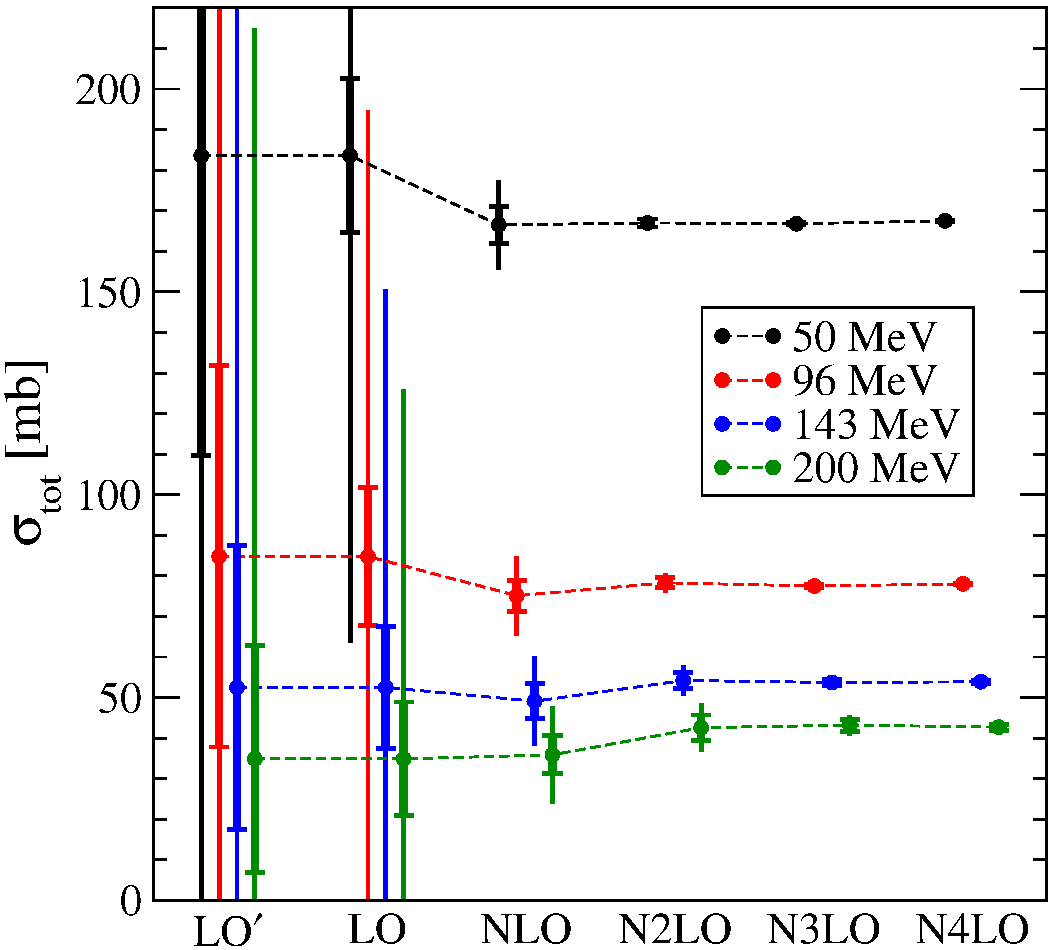
\includegraphics[width=0.5\textwidth]{proposal/doc/images/external/EKM_Tlab_together_setA_eps_approx0.pdf}
  \caption[
    The total proton-neutron scattering cross section
    calculated order by order at different energies
    using chiral potentials
    with 68\% and 95\% degree of belief intervals
    indicated by the thick and thin error bars
    obtained via Bayesian uncertainty quantification.
  ]{
    The total proton-neutron scattering cross section
    calculated order by order at different energies
    using potentials from Ref.~\cite{Epel14ekm2}
    with 68\% and 95\% degree of belief intervals
    indicated by the thick and thin error bars
    obtained via Bayesian uncertainty quantification~\cite{Furn15bayesuq}.
    Figure taken from Ref.~\cite{Furn15bayesuq}.
  }\label{fig:chieft_uq}
\end{figure}

Some comments are now in order regarding interactions as used in this thesis.
The derivation of potentials requires the explicit regularization of momenta
to make divergent integrals over intermediate momenta convergent.
This introduces a dependence on the regularization scheme and scale used,
which is an artifact of the finite order of our EFT.\@
Each additional order in the EFT cancels the scale dependence of the previous order,
and in the limit of infinite order all observables
should not depend on the cutoff scale and scheme used (within reason).
For every interaction used we state the order, the regularization scale,
and the family of interactions, which specifies the regularization scheme used.

We use primarily two families of interactions.
The first set is a family of interactions with NN interactions given up to N3LO
which was worked out by Entem and Machleidt in 2003~\cite{Ente03n3lonn}.
These interactions are denoted by EM when they are used.
The second set was worked out by Entem, Machleidt, and Nosyk in 2017
and provides NN interactions up to N4LO~\cite{Ente17n4lonn}.\@
These interactions are denoted by EMN.\@
From 2007 through 2011, the 3N interactions were worked out~\cite{Ishi07chi3n,Bern07chi3n1,Bern11chi3n2},
and the consistent
(in terms of power-counting and regularization scheme)
3N potentials with these families up to N3LO
were presented in 2015 by Hebeler \textit{et al.}~\cite{Hebe15n3lo3n}.
At N3LO, the chiral power-counting dictates the inclusion of 4N forces
(see Fig.~\ref{fig:chiefttable}).
However, this is generally \textit{not} done
because the inclusion of 4N forces in calculations is prohibitively expensive
and past results have shown that they contribute at the sub-1\%
level~\cite{Tews12neutronmatter4n,Schu18fourbody}.

Chiral EFT essentially resolves all of the shortcomings of phenomenological potentials mentioned previously.
There are still many open questions regarding the derivation of potentials via chiral EFT
and their consistent application in many-body calculations.
For example, there are multiple schools of thought regarding
what the correct power-counting
for nuclear potentials is~\cite{Bean01pertchieft,Nogg05pertchieft,Epel18hownottorenormalize}.
Additionally, the uncertainties from the regularization scheme and scale for nuclear potentials
are still most likely dominant in many-body calculations.
However, the rapid expansion of the range of \abinitio{} calculations over the past two decades has been in no small part
due to the introduction of chiral potentials and the development of auxiliary tools to aid in their application
to many-body calculations.

\section{Similarity renormalization group evolution of nuclear forces}\label{sec:srg}

The similarity renormalization group (SRG) is a method that has been used to great success to ``soften'' nuclear interactions~\cite{Bogn06srg,Wegn94srg,Glaz93srg}.
The key idea of the SRG is the generation of a continuous unitary transformation of a given Hamiltonian,
\begin{equation}
  H(s) = U(s) H U^{\dagger}(s)\,,
\end{equation}
where $s$ is the continuous flow parameter.
The resulting flow equation gives the evolution of the Hamiltonian
\begin{equation}\label{eq:srg_flow_eq}
  \frac{d H(s)}{ds} = [\eta(s), H(s)]\,,
\end{equation}
with $\eta(s) = U(s) d U^{\dagger}(s)/ ds$ and we choose $H(0) = H$.
An ``appropriate'' choice of the anti-Hermitian generator $\eta$
can generate a unitary transformation
such that $H(s)$ evolves, for example, towards a diagonal form.
This leads to a decoupling of low- and high-energy states in the Hamiltonian,
allowing for a truncation in momentum space or a discretized basis
without distorting low-energy observables.

The evaluation of the commutator in the SRG flow equation generates higher-body forces in the evolved Hamiltonian,
even if the initial Hamiltonian consists only of two- and three-body forces.
This means that the fully unitary SRG evolution of an $A$-body Hamiltonian
requires the evaluation of the flow equation in the $A$-body basis.
For all but the smallest systems, this is computationally infeasible.

A pragmatic approach uses the SRG restricted to the three-body space
to evolve two- and three-body nuclear forces to ``softer'' forms in momentum space~\cite{Hebe12srg3n},
reducing coupling between low- and high-energy states.
These evolved potentials are for few-body purposes equivalent to the un-evolved (``bare'') ones,
reproducing the few-body binding energies, radii, and NN phase shifts exactly.
After truncating the potentials, taking advantage of the decoupling,
the few-body observables remain essentially unchanged,
and the low-energy NN phase shifts are also preserved.

The typical choice for the generator in the so-called ``free space'' SRG in nuclear applications is
\begin{equation}
  \eta(s) = [T_{\text{rel}}, H(s)]\,,
\end{equation}
where $T_{\text{rel}}$ is the relative kinetic energy of the two- and three-body systems.
In two-body Jacobi momentum coordinates, $T_{\text{rel}}$ is diagonal,
thus the right-hand side of the flow equation clearly has a fixed point if $H(s)$ is ever diagonal.
Evaluating the flow equation in momentum space in the two-body case for this choice for $\eta$ gives
\begin{equation}
  \frac{dV_2(s; p, p')}{ds} = - {(p^2 - {p'}^2)}^2 V_2(s; p, p') + \int dp'' (p^2 + {p'}^2 - 2 {p''}^2) V_2(s; p, p'') V_2(s; p'', p')\,,
\end{equation}
where $p$ and $p'$ are the incoming and outgoing Jacobi momenta of the two-body subsystem
(see Section~\ref{sec:jacobi_ms_rep}).
We also used the conventional choice of leaving the kinetic energy invariant under the SRG evolution.
Empirically, one can see that the first term dominates the evolution for far off-diagonal elements in nuclear applications,
and so
\begin{equation}
  V_2(s; p, p') \approx V_2(0; p, p') \exp(- s {(p^2 - {p'}^2)}^2)\,.
\end{equation}
Using a redefinition of the flow parameter
\begin{equation}
  \lambda = \frac{1}{s^{1/4}}\,,
\end{equation}
which has units of $\text{fm}^{-1}$ and evolves from $\lambda=\infty$ towards 0,
one can see that over the course of the evolution
off-diagonal parts of the potential outside a band of width $\lambda$ begin to be exponentially suppressed~\cite{Jurg07srgdec}.
Looking at Fig.~\ref{fig:srg_evolved_potential}, one can see that this is qualitatively true,
and the desired decoupling between low- and high-momentum states is achieved.

\begin{figure}[t]
  \centering
  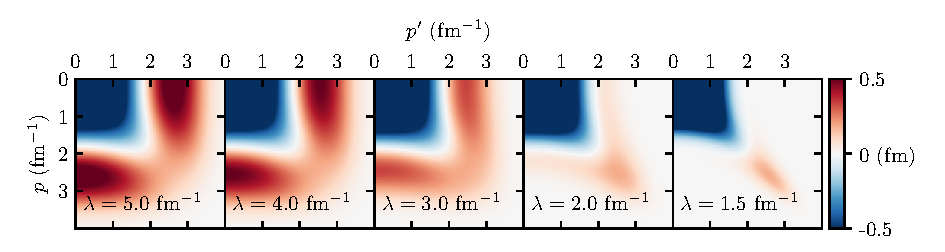
\includegraphics[width=\textwidth]{proposal/doc/images/vnn_srg_emn500_n3lo.pdf}
  \caption[
    An example of an SRG-evolved potential using the chiral EMN NN potential
    at N4LO
    in the ${}^3$S${}_1$ part of the ${}^3$S${}_1$-${}^3$D${}_1$ channel.
  ]{
    An example of an SRG-evolved potential using the chiral NN potential
    from Ref.~\cite{Ente17n4lonn} at N4LO
    in the ${}^3$S${}_1$ part of the ${}^3$S${}_1$-${}^3$D${}_1$ channel.
  }\label{fig:srg_evolved_potential}
\end{figure}

These softened interactions can then be fed into many-body frameworks,
which benefit strongly from the improved convergence with respect to modelspace size.
However, the few-body evolution of potentials neglects induced $A$-body forces,
which do contribute in many-body calculations.
One way to probe the size of the missing many-body forces is to do calculations
with potentials evolved to different values of $s$ or $\lambda$
and see how much the calculated result depends on the renormalization scale.
A strong dependence would indicate significant missing contributions from many-body forces
while no dependence would indicate approximate renormalization group invariance,
which is ultimately the goal~\cite{Bogn09vlowk}.

\section{Representations of nuclear potentials}

The efficient representation of nuclear potentials exploits symmetries of the few-body system and the interactions.
In particular, for 3N forces,
where the potential can depend in principle on 18 parameters in momentum space
($\vec{k}_1$, $\vec{k}_2$, $\vec{k}_3$, $\vec{k}_{1}^{\prime}$, $\vec{k}_{2}^{\prime}$, $\vec{k}_{3}^{\prime}$),
simplifications afforded by these symmetries are essential
to being able to evaluate, store, and calculate with these potentials.

The essential symmetries of the free two- and three-nucleon systems
(from which the potentials are determined)
are
\begin{itemize}
  \item conservation of the center-of-mass momentum of the system,
  \item independence on the center-of-mass momentum,
  \item and rotational invariance~\cite{Hebe20habi}.
\end{itemize}
Additionally, one can simplify things dramatically by making the assumption that the masses of all nucleons are the same,
a reasonable assumption given that the mass difference between the proton and neutron is less than a per mille~\cite{Hebe20habi}.
In this approximation in the absence of electroweak interactions,
the NN force would also be independent of isospin projection,
however the Coulomb interaction breaks this isospin charge symmetry.
Also, even without the Coulomb interaction,
the chiral EFT expansion explicitly breaks isospin charge symmetry at higher orders,
a result of it being constructed in a way
that systematically accounts for the breaking of approximate symmetries.
However, at the orders in chiral EFT considered here,
such isospin charge symmetry violating processes do not contribute.


In the following, we discuss some possible representations of NN forces,
going from one of the representations most convenient for the evaluation of potentials
to the representation of choice for the many-body methods discussed in this thesis.
We mention along the way some of the analogous results for 3N forces.
A more thorough treatment of this topic can be found in Ref.~\cite{Hebe20habi}.

\subsection{Jacobi momentum space}\label{sec:jacobi_ms_rep}

Going from single-particle momenta to Jacobi and center-of-mass momenta,
like
\begin{align}
  \vec{k}_1, \vec{k}_2 & \rightarrow \vec{p}, \vec{P}_{2\text{N}}\,, \\
  \vec{k}_1, \vec{k}_2,\vec{k}_3 & \rightarrow \vec{p}, \vec{q}, \vec{P}_{3\text{N}} \,,
\end{align}
allows one to factor out and ignore the center-of-mass degrees of freedom of the system.
The Jacobi and center-of-mass momenta are defined as
\begin{align}
  \vec{p} &= \frac{\vec{k}_1 - \vec{k}_2}{2}\,,\\
  \vec{P}_{2\text{N}} &= \vec{k}_1 + \vec{k}_2\,,\\
  \vec{q} &= \frac{2\vec{k}_3 - \vec{P}_{2\text{N}}}{3}\,,\\
  \vec{P}_{3\text{N}} &= \vec{k}_1 + \vec{k}_2 + \vec{k}_3\,.
\end{align}
For NN forces, this gives us two-body states of the form
\begin{equation}
  \ket{\vec{p} s_1 m_{s_1} s_2 m_{s_2} t_1 m_{t_1} t_2 m_{t_2}}\,,
\end{equation}
where $s_i=1/2$, $m_{s_i}$, $t_i=1/2$, $m_{t_i}$ are the $i$-th particle's
spin, spin projection, isospin, and isospin projection, respectively.
In cases where explicit values of isospin projection are used,
we adopt the convention that for protons $m_t=1/2$ and for neutrons $m_t=-1/2$.

To take advantage of rotational invariance, one can decompose the potential into partial-wave channels,
with two-body states like
\begin{equation}
  \ket{p \left[l \left(s_1 s_2 \right) S \right] J m_{J} T m_{T}}\,,
\end{equation}
where $p$ is the magnitude of $\vec{p}$,
$l$ is the relative orbital angular momentum of the two-body system,
and $S$, $J$, $m_J$, $T$, $m_{T}$ are the
total spin, total angular momenta, total angular momentum projection, isospin, and isospin projection
of the two-body system.
The resulting potential
\begin{equation}
  \braket{p' \left[l' \left(s_{1}^{\prime} s_{2}^{\prime} \right) S' \right] J' m_{J}^{\prime} T' m_{T}^{\prime}
    | V_{2\text{N}} |
    p \left[l \left(s_{1} s_{2} \right) S \right] J m_{J} T m_{T}
  }\,
\end{equation}
is proportional to $\delta_{JJ'}\delta_{m_J m_{J'}}$ and independent of $m_J$ due to rotational invariance.
Additionally, antisymmetry under exchange of particle indices and parity conservation require
it to also be proportional to $\delta_{S S'} \delta_{T T'}$ with the additional constraints
\begin{align}
  {(-1)}^{l + S + T + 1} & = {(-1)}^{l' + S + T + 1} = 1\,, \\
  l - l' &= -2, 0, 2\,,
\end{align}
and charge conservation requires that it also is proportional to $\delta_{m_T m_{T'}}$.
For notational convenience, we sometimes collect the partial-wave quantum numbers of states
in a collective index $\alpha_2$,
allowing the concise notation for 2N potentials
\begin{equation}
  \braket{p' \alpha_{2}^{\prime}|V_{2\text{N}}| p \alpha_2}\,.
\end{equation}

With this, the representation of NN forces has been reduced to two continuous variables, $p$ and $p'$,
and some strongly constrained partial-wave quantum numbers.
For 3N forces, there is similar simplification possible, yielding three-body states of the form
\begin{equation}
  \ket{p q \left[\left(l S\right) J \left(\ell s\right) j\right] \mathcal{J} \mathcal{M}_{\mathcal{J}} \left(T t\right) \mathcal{T} \mathcal{M}_{\mathcal{T}}}\,,
\end{equation}
where $p$, $l$, $S$, $J$, $T$ still refer to the two-particle subsystem as before,
$q$, $\ell$, $j$ are the Jacobi momentum, orbital angular momentum, and total angular momentum of the third nucleon
relative to the two-body subsystem center-of-mass,
and $s$ and $t$ are the spin and isospin of the third nucleon.
Here, the 3N potential is, among other things, independent of $\mathcal{M}_{\mathcal{T}}$.

\subsection{Jacobi harmonic-oscillator space}

The transformation to Jacobi harmonic-oscillator (HO) space follows quite simply.
Using the radial solutions to the isotropic three-dimensional harmonic oscillator with frequency $\hbar \Omega$,
one obtains
\begin{equation}\label{eq:jacobi_ho_twobody}
  \braket{n' \alpha_{2}^{\prime}|V_{2\text{N}}|n \alpha_2} = \int dp p^2 dp' {p'}^2 R_{n'l'}(p') R_{nl}(p)
  \braket{p' \alpha_{2}^{\prime}|V_{2\text{N}}|p \alpha_2}\,.
\end{equation}
The radial solutions are given by
\begin{equation}
  R_{n l}(p) = \sqrt{\frac{2(n!)}{{(m \hbar \Omega)}^{3/2} \Gamma(n + l + 3/2)}}
  {\left(\widetilde{p}\right)}^{l}
  \exp(- \widetilde{p}^2/2)
  L^{l + 1/2}_{n}\left(\widetilde{p}^2\right)\,,
\end{equation}
where $m$ is the nucleon mass, $\widetilde{p}=p/\sqrt{m \hbar \Omega}$ is the dimensionless momentum,
and $L_{n}^{k}(x)$ are the generalized Laguerre polynomials.
For 3N forces, the Jacobi momenta $q$ and $q'$ must also be transformed, giving two more integrals.

In the infinite modelspace limit, this transformation is exact,
and the dependence on the basis frequency $\hbar \Omega$ disappears.
However, for practical calculations a basis truncation $n_{\text{max}}$ must be introduced,
which implicitly introduces an ultraviolet (UV) cutoff and an infrared (IR) cutoff.
The UV cutoff is due to high frequencies requiring HO wave functions beyond the truncation to be resolved.
The IR cutoff is due to the basis frequency $\hbar \Omega$ setting the minimum frequency reproducable by wave functions in the basis.

For a given truncation,
the optimal $\hbar \Omega$ can be determined by making use of the variational principle,
which states that for the true ground state
the energy functional $E[\ket{\psi}]$ is stationary
under infinitesimal variations of $\ket{\psi}$.
In this case, one can look at the approximate ground state by solving
the two- or three-body system (for example, via exact diagonalization).
For the optimal $\hbar \Omega$, the ground-state energy will be minimal,
guaranteed by the variational principle to be no less than the true ground-state energy.
Many-body calculations are typically done with operators transformed
at several $\hbar \Omega$.
For energies the minimum result under this variation
is taken to be the result of the calculation,
but it is important to note that many many-body methods are \textit{not} variational.

\subsection{Single-particle harmonic-oscillator space}\label{sec:sp_ho}

Many many-body methods used in nuclear physics,
in particular also wave function expansion methods,
work with operators given in a single-particle basis as input.
This means we have a basis of single-particle states
\begin{equation}
  \left\{ \ket{a} \right\}
\end{equation}
spanning the one-body Hilbert space.
Then the set of product states
\begin{equation}
  \ket{a b} = \ket{a} \ket{b}
\end{equation}
spans the two-body Hilbert space.
At this point these states are not appropriately antisymmetrized.
At the end of this section,
we discuss how to recover the required antisymmetry under exchange of particle indices.

In our case, we work with the single-particle harmonic-oscillator basis with the same frequency $\hbar \Omega$
as used in the transformation above.
To be explicit, these states are of the form
\begin{equation}\label{eq:ho_sp_states}
  \ket{n_a \left(l_a s_a\right) j_a m_{j_{a}} t_a m_{t_a}}\,.
\end{equation}
The two-body single-particle states are then
\begin{equation}\label{eq:mscheme_twop_state}
  \ket{n_a \left(l_a s_a\right) j_a m_{j_{a}} t_a m_{t_a} n_b \left(l_b s_b\right) j_b m_{j_b} t_b m_{t_b}}\,,
\end{equation}
or, coupled to two-body total angular momentum $J$,
\begin{equation}\label{eq:jscheme_twop_state}
  \ket{n_a n_b \left[\left(l_a s_a\right) j_a \left(l_b s_b\right) j_b\right]J m_{J} t_a m_{t_a} t_b m_{t_b}}\,.
\end{equation}

To connect the states in Eq.~\ref{eq:mscheme_twop_state} with those in Eq.~\ref{eq:jacobi_ho_twobody},
one does a Talmi-Moshinsky transformation.
This connects the relative and center-of-mass excitation numbers, $n$ and $N$,
and orbital angular momentum numbers, $l$ and $L$,
with the single-particle excitation numbers, $n_a$ and $n_b$,
and orbital angular momentum numbers, $l_a$ and $l_b$.
The central object of this transformation is the harmonic-oscillator bracket
\begin{equation}
  \braket{n_a n_b (l_a l_b) \Lambda | n N (l L) \Lambda}\,,
\end{equation}
where both sets of orbital angular momenta have been coupled to total orbital angular momentum $\Lambda$.
The properties and evaluation of these brackets is discussed in detail in Refs.~\cite{Mosh59hobr,Buck96hobr}.
By appropriately decoupling and recoupling angular momenta
and applying the harmonic-oscillator brackets,
one arrives at NN potential matrix elements of the form
\begin{equation}\label{eq:unsymm_sp_me}
  \braket{ab | V_{2\text{N}} | cd}\,,
\end{equation}
where $a$, $b$, $c$, and $d$ are collective indices
that run over the single-particle states in Eq.~\ref{eq:ho_sp_states}.

The matrix elements in Eq.~\ref{eq:unsymm_sp_me}
do not obey the required antisymmetry of fermions under exchange of particle indices
since the product states $\ket{ab}$ are not antisymmetrized.
Restoring the required antisymmetry,
one obtains the antisymmetrized matrix elements
\begin{align}
  V_{2\text{N},abcd} &= \frac{1}{2}(1 - P_{ab})(1 - P_{cd})\braket{ab | V_{2\text{N}} | cd} \\
  &= (1 - P_{cd}) \braket{ab | V_{2\text{N}} | cd}\,,
\end{align}
where $P_{ab}$ exchanges the indices $a$ and $b$ in the following expression.
The simplification above takes advantage of the symmetry
\begin{equation}
  \braket{ab | V_{2\text{N}} | cd} = \braket{ba | V_{2\text{N}} | dc}\,,
\end{equation}
arising due to the indistinguishability of the two particles.
In the next chapter, we develop the fundamentals of the formalisms
that use these matrix elements as input.



\chapter{Many-body basics and wave function expansion methods}\label{ch:many_body}

The goal of many-body quantum mechanics is to solve
the $A$-body time-independent Sch\"{o}dinger equation.
This requires, among other things, the construction of a set of states that span
the $A$-body Hilbert space.
For distinguishable particles, taking a set of single-particle states $\ket{p}$
and building $A$-body product states $\ket{p_1}\ldots\ket{p_A}$ would be a reasonable approach.
However, the wave function of a system of $A$ nucleons,
which are indistinguishable fermions,
must be antisymmetric under the exchange of any two particle labels.
The explicit antisymmetrization of states going from naive product states
quickly becomes unwieldy with growing $A$.

Second quantization offers an alternative that bakes the required antisymmetry
into the formalism.
This formalism is the basis for a class of many-body methods
called wave function expansion methods, which includes the IM-SRG.\@
These methods have the benefit that,
instead of scaling combinatorially in $A$ like exact diagonalization approaches,
they scale polynomially,
taking advantage of knowledge of a good approximate solution to the ground state
to reduce the task to finding corrections to this zeroth-order ansatz.
In this chapter, we introduce the basics of second quantization and normal ordering,
focusing on the case of fermions.
Then we discuss some of the more traditional wave function expansion methods
before discussing the IM-SRG in detail in the next chapter.

\section{Second quantization}\label{sec:second_quantization}

To consider second quantization, one starts by constructing the Fock space,
the direct sum of all $A$-body antisymmetric Hilbert spaces.
As a concrete example, for the zero-, one-, and two-body Hilbert spaces, we have the bases
\begin{align}
  A = 0 & \rightarrow \ket{0}\,, \\
  A = 1 & \rightarrow \{\ket{p}\}\,, \\
  A = 2 & \rightarrow \left\{\frac{\ket{p}_{1}\ket{q}_{2} - \ket{q}_{1}\ket{p}_2}{\sqrt{2}} \, \Big| \, q > p \right\}\,.
\end{align}
These states (and many more) are all in the Fock space,
related to one another via field operators.

The field operators are particle creation and annihilation operators
that connect states in the $A$-body antisymmetric Hilbert space
to states in the $A+1$-body and $A-1$-body antisymmetric Hilbert spaces.
The creation operator \crea{p} creates a particle in the single-particle state $\ket{p}$.
Operating on an $A$-body state with it creates an $A+1$-body state
with an additional particle in state $\ket{p}$,
\begin{equation}
  \crea{p} \ket{p_1 \ldots p_{A}}_a = (1 - n_{p}) \ket{p p_1 \ldots p_{A}}_a\,,
\end{equation}
where we have explicitly denoted that the states are antisymmetrized.
Here, $n_p$ is the occupation number of state $\ket{p}$ in the $A$-body state,
which for fermions, due to the Pauli exclusion principle, can only be 0 or 1.
Attempting to create a second particle in an already occupied state annihilates the state.

The annihilation operator \annih{p} annihilates a particle in the single-particle state $\ket{p}$.
Operating on an $A$-body state with it creates an $A-1$-body state
with a particle in state $\ket{p}$ removed,
\begin{equation}
  \annih{p} \ket{p p_2 \ldots p_A}_a = n_p \ket{p_2 \ldots p_A}_a\,.
\end{equation}
If no particle with the single-particle state $\ket{p}$ exists in the state,
the annihilation operator annihilates the state.

With the field operators, an antisymmetric $A$-body state can very efficiently be written as
\begin{equation}
  \ket{p_1 p_2 \ldots p_A}_a = \crea{p_1} \crea{p_2} \ldots \crea{p_A} \ket{0}\,.
\end{equation}
This antisymmetrized product of $A$ particles in $A$ unique single-particle states
is frequently referred to as a Slater determinant,
owing to the fact that it can be, in its explicitly antisymmetrized form,
written as an appropriately normalized determinant~\cite{Slat29sladet}.

Since these states should be antisymmetric under exchange of particle indices, that is,
\begin{equation}
  \ket{p_1 p_2 \ldots p_A}_a = - \ket{p_2 p_1 \ldots p_A}_a\,,
\end{equation}
the creation and annihilation operators must anti-commute with themselves,
\begin{align}
  \anticomm{\crea{p}}{\crea{q}} = 0\,,\\
  \anticomm{\annih{p}}{\annih{q}} = 0\,.
\end{align}
Similarly, one can arrive at the anti-commutation relation
between creation and annihiliation operators,
\begin{equation}
  \anticomm{\annih{p}}{\crea{q}} = \delta_{pq}\,.
\end{equation}

With this formalism in place,
we are now in a position to discuss the representation of many-body operators
in the Fock space.
Operators are classified as $A$-body operators if they can at most couple $A$ particles.
We have used this language frequently so far,
but we make it very precise in the following discussion.

Zero-body operators are simple scalars,
\begin{equation}
  \zerobodyop{O} = o\,.
\end{equation}
They have, among other things, in general a non-zero vacuum expectation value.

One-body operators are of the form
\begin{equation}\label{eq:onebody_op_definition}
  \onebodyop{O} = \sum_{pq} \onebodyop{O}_{pq} \crea{p} \annih{q}\,,
\end{equation}
where $\onebodyop{O}_{pq}$ are the matrix elements of $\onebodyop{O}$.
One-body operators have two useful properties.
First, their vacuum expectation value is 0:
\begin{equation}
  \braket{0 | \onebodyop{O} | 0} = 0\,.
\end{equation}
Second, they do not contribute to processes
where the incoming (bra) and outgoing (ket) states differ
in more than one single-particle state.
Some examples of one-body operators are the kinetic energy and an external potential.

Two-body operators are of the form
\begin{equation}
  \twobodyop{O} = \frac{1}{{(2!)}^2} \sum_{pqrs} \twobodyop{O}_{pqrs} \crea{p} \crea{q} \annih{s} \annih{r}\,.\label{eq:twobody_op_definition}
\end{equation}
Here $\twobodyop{O}_{pqrs}$ is an antisymmetrized matrix element, with the property
\begin{equation}
  \twobodyop{O}_{pqrs} = - \twobodyop{O}_{qprs} = - \twobodyop{O}_{pqsr} = \twobodyop{O}_{qpsr}\,.
\end{equation}
We note that in Eq.~\ref{eq:twobody_op_definition}
the order of the annihilation operators is reversed
relative to the indices on the matrix element.
The indices $p$ and $r$ and the indices $q$ and $s$ are ``paired,''
and the product of creation and annihilation operators is structured
such that the pairs are nested inside of eachother,
not adjacent to eachother.
However, by the antisymmetry of the matrix elements,
the matrix element for one pairing determines it
for all other pairings of the same creation and annihilation operators.
Two-body operators have the properties
\begin{align}
  \braket{0 | \twobodyop{O} | 0} & = 0\,,\\
  \braket{p | \twobodyop{O} | q} & = 0\,,
\end{align}
and they do not contribute to processes where incoming and outgoing states
differ in more than two single-particle states.
A typical example of a two-body operator is any pairwise interaction,
such as the Coulomb interaction or NN nuclear forces.

Three-body operators are of the form
\begin{equation}\label{eq:threebody_op_definition}
  \threebodyop{O} = \frac{1}{{(3!)}^2} \sum_{pqrstu} \threebodyop{O}_{pqrstu} \crea{p} \crea{q} \crea{r} \annih{u} \annih{t} \annih{s}\,.
\end{equation}
Here, $\threebodyop{O}_{pqrstu}$ are also antisymmetrized matrix elements, with the property
\begin{equation}
  \threebodyop{O}_{pqrstu} = {(-1)}^{\sigma_1}{(-1)}^{\sigma_2}\threebodyop{O}_{\sigma_1(pqr)\sigma_2(stu)}\,,
\end{equation}
where $\sigma_1$ and $\sigma_2$ are permutations
and the ${(-1)}^{\sigma}$ prefactors account for the signs of the permutations.
Three-body operators have the properties
\begin{align}
  \braket{0 | \threebodyop{O} | 0} & = 0\,,\\
  \braket{p | \threebodyop{O} | q} & = 0\,, \\
  \braket{p q| \threebodyop{O} |r s} & = 0\,,
\end{align}
and they do not contribute to processes where incoming and outgoing states
differ in more than three single-particle states.
Examples of three-body operators are 3N nuclear forces.
These definitions can be generalized to get the general representation of any $A$-body operator,
and the properties follow analogously.

\section{Normal ordering}

A product of creation and annihilation operators is in normal order
if all creation operators appear to the left of all annihilation operators.
The normal ordering operation on $c A$,
where c is a scalar coefficient and $A$ is a product of creation and annihilation operators,
can be written as
\begin{equation}
  \nogen{c A} = {(-1)}^{\sigma} c \sigma(A)\,
\end{equation}
where $\sigma$ is a permutation that rearranges the product $A$ into normal order.
This rearrangement is not unique,
but, since each change in the permutation is accompanied by a change in the exchange prefactor,
all normal-ordered products resulting from different permutations used in normal ordering
are equivalent.
Also, note that in general $\nogen{A} \neq A$,
since anti-commuting creation and annihilation operators past eachother
will leave a residual $\delta_{pq}$ from their anti-commutation relation.

\subsection{General properties}\label{sec:normal_ordering_properties}

Suppose the product of creation and annihilation operators $A$
contains $p$ creation operators and $q$ annihilation operators.
Then, unless $p$ and $q$ are both 0,
$\nogen{A}$ has a vacuum expectation value of 0.
Additionally, $\nogen{A}$ does not contribute to processes
where the incoming state has less than $q$ particles
or the outgoing state has less than $p$ particles.

We are now interested in considering products of normal-ordered products
of creation and annihilation operators.
Ultimately, we will use Wick's theorem to systematically evaluate these products~\cite{Wick50wickthm}.
To introduce the theorem, we first need to introduce the notion of a Wick contraction,
which for adjacent operators $\alpha$ and $\beta$ is defined as
\begin{equation}
  \acontraction{}{\alpha}{}{\beta}
  \alpha \beta = \alpha \beta - \nogen{\alpha \beta}\,.
\end{equation}
The value of the contraction is the vacuum expectation value of $\alpha \beta$.
Note that for two operators that are already in normal order their contraction vanishes.
This provides an alternative definition of normal ordering,
namely a product of two operators is in normal order
if its vacuum expectation value is 0
and so its contraction vanishes.
This leads to an extension of normal ordering
that works for many different vacuum choices,
including multi-reference vacuums
which we don't consider any further in this work~\cite{Kutz97mrno}.

We are now equipped to use Wick's theorem
to rewrite a general product of creation and annihilation operators
in terms of sums of normal-ordered products and contractions:
\begin{equation}\label{eq:wicks_theorem}
  \begin{split}
    ABCDEF\ldots =& \nogen{ABCDEF\ldots} \\
    & + \acontraction{}{A}{}{B} AB \,\nogen{CDEF\ldots} - \acontraction{}{A}{}{C} AC \,\nogen{BDEF\ldots} + \text{singles}\\
    &+ \left(\acontraction{}{A}{}{B} AB \acontraction{}{C}{}{D} CD
    - \acontraction{}{A}{}{C} AC \acontraction{}{B}{}{D} BD
    + \acontraction{}{A}{}{D} AD \acontraction{}{B}{}{C} BC\right) \, \nogen{EF\ldots} + \text{doubles} \\
    &+ \cdots + \text{full contractions}\,.
  \end{split}
\end{equation}
The minus signs arise due to the fact that in order to simplify the contraction
and pull it out of the normal-ordered product,
we must anti-commute the contracted operators such that they are adjacent.

The generalized Wick's theorem states that
for a product of two normal-ordered products of creation and annihilation operators,
$A=\nogen{A_1 A_2 \ldots A_N}$ and $B=\nogen{B_1 B_2 \ldots B_M}$,
the resulting expression in terms of normal-ordered products
is the sum of all normal-ordered terms with 0 to $\text{min}(N, M)$ contractions
between the operators in $A$ and $B$, that is,
\begin{equation}\label{eq:gen_wicks_theorem}
  \begin{split}
    \nogen{A_1 A_2 \ldots A_N} \nogen{B_1 B_2 \ldots B_M} = &
    \nogen{A_1 A_2 \ldots A_N B_1 B_2 \ldots B_M} \\
    & + {(-1)}^{N-1} \acontraction{}{A_1}{}{B_1} A_1 B_1 \nogen{A_2 \ldots A_N B_2 \ldots B_M} \\
    & + {(-1)}^{N-2} \acontraction{}{A_2}{}{B_1} A_2 B_1 \nogen{A_1 \ldots A_N B_2 \ldots B_M} \\
    & + {(-1)}^{N} \acontraction{}{A_1}{}{B_2} A_1 B_2 \nogen{A_2 \ldots A_N B_1 \ldots B_M} \\
    & + {(-1)}^{N-1} \acontraction{}{A_2}{}{B_2} A_2 B_2 \nogen{A_1 \ldots A_N B_1 \ldots B_M} \\
    & + \text{singles} + \text{doubles} + \cdots\,.
  \end{split}
\end{equation}
Despite the name, this is a special case of Eq.~\ref{eq:wicks_theorem}.

\subsection{Vacuum normal ordering}

In Section~\ref{sec:normal_ordering_properties},
we discussed the properties of normal ordering in general,
and while we referenced ``the vacuum'' several times
(for example, in the context of vacuum expectation values),
we never specified the specific vacuum involved.
Indeed, normal ordering is dependent on the vacuum with respect to which it is done,
and there are multiple options for this vacuum.
In the following, we focus on normal ordering
with respect to the \textit{physical} vacuum $\ket{0}$,
that is, the state with no particles present.

The fermion creation and annihilation operators \crea{p} and \annih{p}
are the \textit{physical} creation and annihilation operators,
so normal ordering with respect to the physical vacuum,
which we denote by \novac{\ldots},
produces products with all creation operators to the left of annihilation operators.
Concretely, one can consider adjacent Wick contractions,
which should be 0 for pairs of operators already in normal order.
Applying the definition that a contraction of two adjacent operators
is the vacuum expectation value of the operator product,
we find
\begin{equation}
  \bcontraction{}{\annih{p}}{}{\crea{q}} \annih{p}\crea{q} = \braket{0|\annih{p} \crea{q} | 0} = \delta_{pq}\,,
\end{equation}
where we use the contraction \textit{below}
to indicate that we are normal ordering with respect to the physical vacuum.
Similarly, we find
\begin{align}
  \bcontraction{}{\annih{p}}{}{\annih{q}} \annih{p}\annih{q} &= 0\,, \\
  \bcontraction{}{\crea{p}}{}{\crea{q}} \crea{p}\crea{q} &= 0\,, \\
  \bcontraction{}{\crea{p}}{}{\annih{q}} \crea{p}\annih{q} &= 0\,,
\end{align}
indicating that these products are already in normal order, as expected.

As a brief aside,
the definitions for the second-quantized form of one-, two-, and three-body operators
in Eqs.~\ref{eq:onebody_op_definition},~\ref{eq:twobody_op_definition}, and~\ref{eq:threebody_op_definition}
are clearly already in normal order with respect to the physical vacuum.
This is no longer the case when we normal order with respect to some other vacuum.

\subsection{In-medium normal ordering}

One alternative is normal ordering with respect to an $A$-body reference state,
also called the Fermi vacuum,
given by
\begin{equation}\label{eq:ref_state_defintion}
  \refgnd = \prod_{i=1}^A \crea{p_i} \ket{0}\,.
\end{equation}
The frequently used occupation numbers for single-particle states in the reference state $n_p$
are then
\begin{equation}
  n_p =
  \begin{cases}
    1 & p \in \{p_i\}\,, \\
    0 & p \not\in \{p_i\}\,.
  \end{cases}
\end{equation}
When calculating operator matrix elements for an $A$-body system,
every bra or ket state comes with $A$ annihilation or creation operators
along with the physical vacuum.
A more practical, but equivalent way to go about this is constructing
$A$-body states from the reference state \refgnd,
annihilating states occupied in the reference state but unoccupied in the state of interest
and creating in their place particles occupied in the state of interest.
As an example, an $A$-body state that differs from the reference state
by one single-particle state is given by
\begin{equation}
  \crea{a} \annih{i} \refgnd \equiv \refhp{i}{a}\,.
\end{equation}

One thing to note is that with respect to the reference state,
the fermion creation and annihilation operators no longer have certain useful properties.
For example, the annihilation operator no longer always annihilates the Fermi vacuum,
and the creation operator in some cases \textit{does} annihilate the Fermi vacuum.
However, one can define quasiparticle creation and annihiliation operators
that recover these properties with respect to the reference state,
with the annihilation operator given by
\begin{equation}
  \qpannih{p} =
  \begin{cases}
    \annih{p} & \text{if $p$ is unoccupied in the reference state,} \\
    \crea{p} & \text{if $p$ is occupied in the reference state,}
  \end{cases}
\end{equation}
and the creation operator being related by conjugation.

These quasiparticle field operators obey all the typical anti-commutation relations
and have the usual properties, just with respect to the reference state:
\begin{align}
  \anticomm{\qpannih{p}}{\qpcrea{q}} &= \delta_{pq}\,,\\
  \anticomm{\qpannih{p}}{\qpannih{q}} & = 0 \,, \\
  \anticomm{\qpcrea{q}}{\qpcrea{q}} &= 0\,, \\
  \qpannih{p} \refgnd &= 0\,, \\
  \qpcrea{p} \refgnd & \neq 0\,.
\end{align}
The quasiparticle creation operator $\qpcrea{p}$
annihilates a particle in the reference state if the state $p$ is occupied,
producing a so-called \text{hole} state.
But when $p$ is unoccupied in the reference state,
$\qpcrea{p}$ creates a particle.
This gives this formalism its name, the particle-hole formalism.

In this thesis so far,
we have used indices $p$, $q$, $r$, \ldots\ to indicate that
the indices run over all single-particle states.
Here we introduce the convention that the indices $i$, $j$, $k$, \ldots\
only run over hole states, that is, states that are occupied in the reference state,
and the indices $a$, $b$, $c$, \ldots\ only run over particle states,
that is, states that are unoccupied in the reference state.

We are now interested in normal ordering with respect to our reference state,
which we denote by \noref{\ldots} and with contractions above the operators.
This can be accomplished via Wick's theorem (see Eq.~\ref{eq:wicks_theorem}).
We only need to know the values of different Wick contractions.
For our quasiparticle field operators, we find
\begin{align}
  \acontraction{}{\qpannih{p}}{}{\qpcrea{q}} \qpannih{p}\qpcrea{q} & =  \delta_{pq}\,, \\
  \acontraction{}{\qpannih{p}}{}{\qpannih{q}} \qpannih{p}\qpannih{q} &= 0\,, \\
  \acontraction{}{\qpcrea{p}}{}{\qpcrea{q}} \qpcrea{p}\qpcrea{q} &= 0\,, \\
  \acontraction{}{\qpcrea{p}}{}{\qpannih{q}} \qpcrea{p}\qpannih{q} &= 0\,,
\end{align}
exactly the same as for the physical field operators
when normal ordering with respect to the physical vacuum.

The case of physical field operators is more relevant to us,
since our operators are given in terms of physical creation and annihilation operators.
For the physical field operators, we find
\begin{align}
  \acontraction{}{\annih{p}}{}{\crea{q}} \annih{p}\crea{q} & = (1 - n_p) \delta_{pq}\,, \\
  \acontraction{}{\annih{p}}{}{\annih{q}} \annih{p}\annih{q} &= 0\,, \\
  \acontraction{}{\crea{p}}{}{\crea{q}} \crea{p}\crea{q} &= 0\,, \\
  \acontraction{}{\crea{p}}{}{\annih{q}} \crea{p}\annih{q} &= n_p \delta_{pq}\,.
\end{align}

Assuming we have a Hamiltonian with one-, two-, and three-body operators,
\begin{equation}\label{eq:standard_threebody_free_hamiltonian}
  H = \onebodyop{H} + \twobodyop{H} + \threebodyop{H}\,,
\end{equation}
we can normal order it with respect to our reference state
by making use of Eq.~\ref{eq:wicks_theorem} and the contractions above.
Doing this yields the following expression for our normal-ordered Hamiltonian:
\begin{align}
  \hnozero &= \sum_i \onebodyop{H}_{ii} + \frac{1}{2}\sum_{ij} \twobodyop{H}_{ijij} + \frac{1}{6} \sum_{ijk} \threebodyop{H}_{ijkijk}\,, \\
  \hnoone_{pq} &= \onebodyop{H}_{pq} + \sum_i \twobodyop{H}_{piqi} + \frac{1}{2} \sum_{ij} \threebodyop{H}_{pijqij} \,, \\
  \hnotwo_{pqrs} &= \twobodyop{H}_{pqrs} + \sum_i \threebodyop{H}_{pqirsi} \,,  \\
  \hnothree_{pqrstu} &= \threebodyop{H}_{pqrstu} \,.
\end{align}
With this we have normal ordered our Hamiltonian with respect to our reference state,
obtaining our normal-ordered Hamiltonian.
Additionally, we can bring any products of normal-ordered operators to a normal-ordered form
by applying the generalized Wick's theorem.

At this point, a few comments are in order about the choice of our reference state \refgnd.
The choice of reference state corresponds to a partitioning of our Hamiltonian
into a part that is exactly solved by the reference state
and a part that contributes corrections to this zeroth-order solution,
schematically
\begin{equation}
  H = H_0 + H_1\,,
\end{equation}
as in perturbation theory.
A reasonable choice for the reference state corresponds to a choice
that solves a problem ``approximately'' like the problem of interest,
for example a spherical harmonic oscillator for spherical bound systems.
The normal-ordered zero-body part of the Hamiltonian \hnozero{}
is the expectation value of the ground-state energy as a result of the partitioning.
\hnoone, \hnotwo, and \hnothree{} do not contribute to this expectation value by construction.
To improve the approximation of the physical ground state,
one can:
\begin{enumerate}
  \item improve the reference state, as is discussed in Section~\ref{sec:hartree_fock},
  \item and/or include corrections to the ground-state wave function,
    for example admixtures of one-particle one-hole excited states \refhp{i}{a},
    as is discussed in Section~\ref{sec:mbpt}.
\end{enumerate}

\section{The Hartree-Fock method}\label{sec:hartree_fock}

The variational principle states that the true ground state $\ket{\psi}$
globally minimizes the energy functional
\begin{equation}
  E[\ket{\psi}] = \frac{\braket{\psi | H | \psi}}{\braket{\psi|\psi}}\,.
\end{equation}
However, the ground state will in general not be describable by a single Slater determinant,
meaning that cannot hope to get the exact ground-state energy
by normal ordering our Hamiltonian with respect to some optimized reference state.
Still, one can optimize the reference state
within a space restricted to Slater determinants
to get the best possible single Slater determinant approximation to the ground state.

This is the core idea behind the Hartree-Fock method~\cite{Slat28hf,Fock30hf,Hart28hf}.
Working from a known single-particle basis $\ket{p}$,
one wants to find a new single-particle basis $\ket{p'}$
such that our reference state
\begin{equation}
  \refgnd = \ket{p_{1}^{\prime} \ldots p_{A}^{\prime}}
\end{equation}
has the minimal energy expectation value, or Hartree-Fock energy,
\begin{equation}
  \braket{\Phi | H | \Phi} = \hnozero\,.
\end{equation}
Rewriting the optimized basis in terms of our original basis,
\begin{equation}
  \ket{p'} = \sum_{p'p}C_{p'p} \ket{p}\,,
\end{equation}
where $C$ is a unitary matrix giving the basis transformation,
we can expand the Hartree-Fock energy
using our Hamiltonian from Eq.~\ref{eq:standard_threebody_free_hamiltonian} as
\begin{equation}
  \hnozero = \sum_{i'} \onebodyop{H}_{i'i'} + \frac{1}{2}\sum_{i'j'} \twobodyop{H}_{i'j'i'j'}
  + \frac{1}{6}\sum_{i'j'k'} \threebodyop{H}_{i'j'k'i'j'k'}\,,
\end{equation}
where these matrix elements can be connected back to those in our known single-particle basis,
\begin{align}
  \onebodyop{H}_{i'i'} &= \sum_{pq} C_{pi'}^{*} \onebodyop{H}_{pq} C_{q i'}\,,\\
  \twobodyop{H}_{i'j'i'j'} &= \sum_{pqrs} C_{pi'}^{*}C_{qj'}^{*} \twobodyop{H}_{pqrs} C_{r i'}C_{s j'}\,,\\
  \threebodyop{H}_{i'j'k'i'j'k'} &= \sum_{pqrstu} C_{pi'}^{*}C_{qj'}^{*}C_{rk'}^{*} \threebodyop{H}_{pqrstu} C_{s i'}C_{t j'}C_{u k'}\,.
\end{align}
The minimization of $\hnozero$ gives the Hartree-Fock equations,
\begin{equation}
  \sum_{q} F_{pq} C_{qr} = C_{pr} e_{r}\,,
\end{equation}
where $F_{pq}$ is the Fock matrix given by
\begin{equation}\label{eq:fock_matrix_pre}
  F_{pq} = \onebodyop{H}_{pq} + \sum_{rsj'} C_{rj'}^{*} \twobodyop{H}_{prqs} C_{s j'} + \frac{1}{2}\sum_{rstu j'k'} C_{rj'}^{*}C_{sk'}^{*} \threebodyop{H}_{prsqtu} C_{t j'}C_{u k'}\,,
\end{equation}
and $e_i$ are Lagrange multipliers
ensuring orthonormality of the new single-particle basis.
Using that
\begin{equation}\label{eq:hf_density_update}
  \sum C_{p, i'}^{*} C_{q, i'} = \rho_{pq}\,,
\end{equation}
the one-body density in the known single-particle basis,
we can simplify Eq.~\ref{eq:fock_matrix_pre} to
\begin{equation}\label{eq:fock_matrix}
  F_{pq} = \onebodyop{H}_{pq} + \sum_{rs} \rho_{rs} \twobodyop{H}_{prqs} + \frac{1}{2}\sum_{rstu}\rho_{rt} \rho_{su} \threebodyop{H}_{prsqtu}\,.
\end{equation}

These equations are solved self-consistently,
where in each iteration $k$:
the density $\rho^{(k-1)}$ of the previous iteration
is used to construct the new Fock matrix $F^{(k)}$,
$F^{(k)}$ is diagonalized,
a new $C^{(k)}$ is constructed from the eigenvectors of $F^{(k)}$,
and the density $\rho^{(k)}$ is constructed via Eq.~\ref{eq:hf_density_update}.
To start, we choose $\rho^{(0)}_{pq} = n_p \delta_{pq}$.
The iteration terminates when between iterations
the $e_{i}^{(k)}$ change by less than some threshold.
At this point, we can transform all operators to our new optimized single-particle basis
by applying $C$ appropriately.
After this transformation $\hnoone$ is diagonal with diagonal matrix elements $e_i$,
the single-particle energies.

\section{Many-body perturbation theory}\label{sec:mbpt}

Many-body perturbation theory (MBPT) has its formal roots in formal perturbation theory,
which abstractly gives the perturbation theory formalism.
MBPT then specifies certain details about the system
and the starting point for perturbation theory
and translates the formalism into concrete formulas
for order-by-order corrections to the wave function and the energy of a state.
In this section we give the key results from formal perturbation theory,
discuss the setup for MBPT,
and give the formulas for second- and third-order MBPT corrections to the energy.
We refer the interested reader to Refs.~\cite{Shav09mbpt_cc_book,Tich20mbptreview}
for a more comprehensive treatment.

To start, one partitions the Hamiltonian
\begin{equation}
  H = H_0 + H_1\,,
\end{equation}
into $H_0$,
for which the solution to the Schr\"{o}dinger equation is known exactly
with solutions $\ket{\Phi_k}$ and corresponding energies $E^{(0)}_{k}$,
and a perturbation $H_1$.
One is interested in an expansion of the true eigenstate $\ket{\Psi_k}$
in terms of the unperturbed solutions $\ket{\Phi_k}$.
We concentrate our discusion here on an expansion for the ground state,
so the ground state of $H$ is denoted $\ket{\Psi}$
and the ground state of $H_0$,
the starting point of the expansion,
is denoted $\refgnd$ with an unperturbed energy $E^{(0)}$.

The partitioning comes with the definition of the projection operators
\begin{align}
  P &= \ket{\Phi}\bra{\Phi}\,, \\
  Q &= \sum_{k\neq 0}\ket{\Phi_k}\bra{\Phi_k}\,.
\end{align}
Working with the so-called intermediate normalization
\begin{equation}
  \braket{\Psi|\Phi} = 1\,,
\end{equation}
one can write the ground state of $H$ as
\begin{align}
  \ket{\Psi} &= (P + Q)\ket{\Psi} \\
  &= \refgnd + \ket{\chi}\,,
\end{align}
where $\ket{\chi} = Q \ket{\Psi}$ is what needs to be solved for.

The result of formal perturbation theory is that
using the Rayleigh-Schr\"{o}dinger resolvent
\begin{equation}
  R = \sum_{k\neq 0} \frac{\ket{\Phi_k}\bra{\Phi_k}}{E^{(0)} - E^{(0)}_{k}} \,
\end{equation}
the correction to the unperturbed ground state is given by
\begin{equation}
  \ket{\chi} = \sum_{n=1}^{\infty}{(R H_1)}^n \refgnd_c\,,
\end{equation}
where the `$c$' subscript indicates that the expansion is connected,
which ensures its size extensivity,
that is, that calculated observables scale linearly with the size of the system.
The corrections to the energy beyond the standard first-order energy correction
\begin{equation}
  E^{(1)} = \braket{\Phi | H_1 | \Phi}\,,
\end{equation}
are given by
\begin{align}
  \Delta E &= \braket{\Phi | H_1 | \chi} \\
          &= \bra{\Phi}  H_1 \sum_{n=1}^{\infty}{(R H_1)}^n \refgnd_c\,.
\end{align}
As an example, the second-order correction to the energy is
\begin{equation}
  E^{(2)} = \sum_{k\neq 0} \frac{\braket{\Phi | H_1 | \Phi_k}\braket{\Phi_k | H_1 | \Phi}}
  {E^{(0)} - E^{(0)}_k}\,.
\end{equation}
This makes it clear that the corrections to the ground state involve
the perturbation $H_1$ connecting the unperturbed ground state in the $P$-space
to excited states in the $Q$-space before connecting these back to the ground state.

Transitioning to (single-reference) many-body perturbation theory,
we define our $A$-body Hilbert space as comprising our reference state
and $n$-particle $n$-hole excitations of the reference state:
\begin{equation}
  \{\refgnd, \refhp{i}{a}, \refhp{ij}{ab}, \refhp{ijk}{abc}, \ldots \}\,.
\end{equation}
After normal ordering with respect to $\refgnd$,
we have our normal-ordered zero- through three-body operators,
$\hnozero$, $\hnoone$, $\hnotwo$, and $\hnothree$.
This choice of basis corresponds to the following partitioning:
our unperturbed Hamiltonian is
\begin{align}
  H_0 &= \hnozero + \text{diag}(\hnoone) \\
      &= \hnozero + \sum_{p} e_p \noref{\crea{p} \annih{p}}\,,
\end{align}
where $e_p = \hnoone_{pp}$ are the single-particle energies.
The energy of the reference state is given by $\hnozero$.
The energy of an $n$-particle $n$-hole excited state $\refhp{ij\cdots}{ab\cdots}$ is given by
\begin{equation}
  \hnozero + \epsilon_{ij\cdots}^{ab\cdots}
\end{equation}
with
\begin{equation}\label{eq:mp_energy_denom}
  \epsilon_{ij\cdots}^{ab\cdots} = (e_a + e_b + \cdots) - (e_i + e_j + \cdots)\,.
\end{equation}
The perturbation is then
\begin{equation}
  H_1 = \hnoone - \text{diag}(\hnoone) + \hnotwo + \hnothree\,.
\end{equation}
Finally, the many-body resolvent is
\begin{equation}\label{eq:mbpt_resolvent}
  R = -\sum_{ai} \frac{\refhp{i}{a}\bra{\Phi_{i}^{a}}}{\epsilon_{i}^{a}}
      -\frac{1}{{(2!)}^2} \sum_{abij}\frac{\refhp{ij}{ab}\bra{\Phi_{ij}^{ab}}}{\epsilon_{ij}^{ab}}
      -\frac{1}{{(3!)}^2} \sum_{abcijk}\frac{\refhp{ijk}{abc}\bra{\Phi_{ijk}^{abc}}}{\epsilon_{ijk}^{abc}}
      + \ldots \,.
\end{equation}

We are now in a position to discuss the second- and third-order contributions to the ground-state energy.
Using Eq.~\ref{eq:mbpt_resolvent} and the properties of normal-ordered operators,
the second-order correction to the ground-state energy is given by
\begin{equation}
    E^{(2)} = -\sum_{ai} \frac{\hnoone_{ai}\hnoone_{ia}}{\epsilon_{i}^{a}}
      -\frac{1}{{(2!)}^2} \sum_{abij}\frac{\hnotwo_{abij}\hnotwo_{ijab}}{\epsilon_{ij}^{ab}}
      -\frac{1}{{(3!)}^2} \sum_{abcijk}\frac{\hnothree_{abcijk}\hnothree_{ijkabc}}{\epsilon_{ijk}^{abc}}\,.
\end{equation}
The first term in this equation is related to a so-called non-canonical diagram
that vanishes if we choose the Hartree-Fock (HF) reference state to be our determinant.
This is because, as mentioned previously, $\hnoone$ is by definition diagonal in the HF basis.

\begin{figure}[t!]
  \centering
  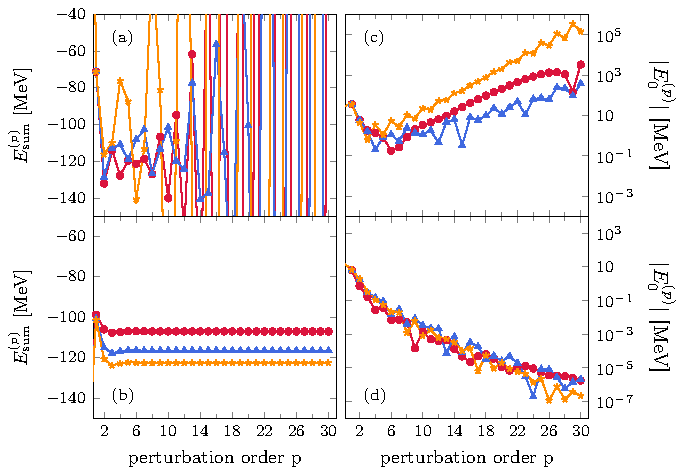
\includegraphics[width=0.8\textwidth]{proposal/doc/images/external/ho_vs_hf_mbpt.pdf}
  \caption[
    The partial sums (left) and order-by-order contributions (right)
    for an MBPT calculation of the ground-state energy of ${}^{16}\text{O}$
    using a harmonic-oscillator reference state (top)
    and a Hartree-Fock reference state (bottom).
    The red, blue, and yellow points are for $N_{\text{max}}=2$, 4, and 6,
    the basis truncation parameter for the approach used.
  ]{
    The partial sums (left) and order-by-order contributions (right)
    for an MBPT calculation of the ground-state energy of ${}^{16}\text{O}$
    using a harmonic-oscillator reference state (top)
    and a Hartree-Fock reference state (bottom).
    The red, blue, and yellow points are for $N_{\text{max}}=2$, 4, and 6,
    the basis truncation parameter for the approach used.
    Figure taken from Ref.~\cite{Tich16hohfmbpt}.
  }\label{fig:ho_vs_hf_mbpt}
\end{figure}

At the third order, even considering only canonical diagrams,
the number of diagrams possible with two- and three-body operators grows to 17.
The complete list of these diagrams can be found in Ref.~\cite{Hu18mbptthreebody}.
The canonical contributions involving only the normal-ordered two-body Hamiltonian are
\begin{equation}
  \begin{split}
  E^{(3)}_{\text{2-body only}} =
    &\frac{1}{8} \sum_{abcdij} \frac{\hnotwo_{ijab} \hnotwo_{abcd}\hnotwo_{cdij}}{\epsilon_{ij}^{ab}\epsilon_{ij}^{cd}} \\
    &+ \frac{1}{8} \sum_{abijkl} \frac{\hnotwo_{ijab} \hnotwo_{abkl}\hnotwo_{klij}}{\epsilon_{ij}^{ab}\epsilon_{kl}^{ab}} \\
    &- \sum_{abcijk} \frac{\hnotwo_{ijab} \hnotwo_{kbic}\hnotwo_{ackj}}{\epsilon_{ij}^{ab}\epsilon_{kj}^{ac}}\,.
  \end{split}
\end{equation}
The complete set of non-canonical third-order contributions
with only one- and two-body operators
is given, among other places, in Ref.~\cite{Tich17phd}.

The inclusion of additional terms is not the only challenge when dealing with a non-canonical reference state.
Choosing a different reference state than the HF determinant
corresponds to choosing a worse partitioning for $H$,
that is, more information is held in the perturbation $H_1$,
as the the HF determinant is the best possible single Slater determinant approximation
to the ground state.
This less optimal choice can lead to poor convergence behavior of MBPT~\cite{Tich16hohfmbpt}.
For instance, in Fig.~\ref{fig:ho_vs_hf_mbpt}
the ground-state energy of ${}^{16}\text{O}$ was calculated
using a harmonic-oscillator determinant and a Hartree-Fock determinant
for the reference state.
While for the HF reference state MBPT converges nicely,
for the HO reference state the calculation rapidly begins to diverge
when going to higher orders in perturbation theory.
Additionally,
while MBPT benefits strongly from working with SRG-evolved Hamiltonians,
it can have difficulty converging even when using an HF reference state
for bare nuclear Hamiltonians that are too ``hard''~\cite{Tich20mbptreview}.

\section{Non-perturbative techniques}

The convergence challenges of MBPT motivate us to consider non-perturbative many-body methods,
which sum to all orders certain types of diagrams to produce a convergent result.
Coupled cluster theory and the in-medium similarity renormalization group
are two examples of such methods.
Their non-perturbative nature makes them less sensitive to the choice of reference state
(although convergence speed will be affected by a non-canonical choice of reference state)
and better able to deal with ``harder'' nuclear Hamiltonians.
We discuss the IM-SRG in detail in the next chapter.
Here, we aim to briefly introduce the coupled cluster many-body approach
as it shares many similarities with the IM-SRG.\@

The ansatz for the coupled cluster (CC) approach is describing the ground state as
\begin{equation}
  \ket{\Psi} = \exp(T)\ket{\Phi}\,,
\end{equation}
where $T$ is the cluster operator,
which when applied exponentially to the reference state $\refgnd$ yields the ground state~\cite{Hage13ccreview}.
$T$ contains in general one- through $A$-body operators,
\begin{equation}
  T = \onebodyop{T} + \twobodyop{T} + \cdots + \abodyop{T}\,,
\end{equation}
which generate particle-hole excitations of the reference state.

The ground-state energy is then given by
\begin{align}
  E &= \braket{\Psi | H | \Psi} \\
  &= \braket{\Phi | \exp(-T) (\hnoone + \hnotwo + \hnothree) \exp(T) | \Phi} + \hnozero \\
  &\equiv \braket{\Phi | \overline{H} | \Phi} + \hnozero\,,
\end{align}
where we have defined the similarity-transformed Hamiltonian $\overline{H}$.
The task is to solve for matrix elements of the different $A$-body parts of $T$
such that
\begin{equation}
  0 = \braket{\Phi_{ijk\ldots}^{abc\ldots} | \overline{H} | \Phi}\,
\end{equation}
for all $n$-particle $n$-hole excited states of the reference state.
These are the coupled cluster equations.

One computes $\overline{H}$ via the Baker-Campbell-Hausdorff expansion,
\begin{equation}
  \overline{H} = H_N + \comm{H_N}{T} + \frac{1}{2!} \comm{\comm{H_N}{T}}{T} + \ldots \,,
\end{equation}
where $H_N=\hnoone + \hnotwo + \hnothree$.
This commutator expansion ensures that only connected diagrams in the MBPT expansion are generated,
ensuring the size-extensivity of the method.
A standard approach in nuclear physics is to truncate $T$, $H_N$, and the commutator
at the two-body level,
giving two coupled cluster equations
\begin{align}
  0 &= \braket{\Phi_{i}^{a} | \overline{H} | \Phi}\,,\\
  0 &= \braket{\Phi_{ij}^{ab} | \overline{H} | \Phi}\,,
\end{align}
known as CCSD (SD for singles and doubles).
Another variant approximately treats the so-called triples and is denoted CCSD(T).\@
In the next chapter, when discussing the IM-SRG,
the many similarities of the methods will be quite obvious.



\include{proposal/doc/03_imsrg_for_nuclear_structure}

\chapter{Results}\label{ch:results}

In this chapter, we discuss the application of the IM-SRG
to calculate the ground-state energies of two different fermionic systems.
The first is the pairing Hamiltonian,
which has been used to study pairing effects in finite and infinite systems.
We use this well-studied system as a benchmark for our numerical implementation,
as its small modelspace allows for calculations to complete relatively quickly.
The second is ${}^4\text{He}$,
the lightest closed-shell nucleus,
in a restricted modelspace in the IM-SRG(2).
The results of our implementation are then compared
against those from another open-source IM-SRG(2) library.

\section{The pairing Hamiltonian}

The pairing Hamiltonian is given by
\begin{equation}\label{eq:pairing_hamiltonian}
  H = \delta \sum_{p\sigma} (p - 1) \crea{p\sigma} \annih{p\sigma}
  - \frac{g}{2} \sum_{p q} \crea{p+}\crea{p-} \annih{q-} \annih{q+}\,,
\end{equation}
where we have equally-spaced two-fold degenerate levels indexed by the quantum number $p$
and an attractive (for $g > 0$) pairing interaction.
Cooper first considered this Hamiltonian in 1956~\cite{Coop56pairing_hamiltonian},
which led to the successful Bardeen-Cooper-Schreifer (BCS) theory of superconductivity~\cite{Bard57bcs}.
The exact eigenvalues of the pairing Hamiltonian were given by Richardson in 1963,
where the solutions are obtained via the solution of the non-linear coupled Richardson equations~\cite{Rich63pairing_hamiltonian}.

We focus on a restricted case where $p=1,\ldots,4$ and $\delta=1\mev$,
and we vary the strength of the pairing interaction $g$.
We are interested in the ground state of four fermions,
for which our reference state is the state with the two lowest levels completely filled,
\begin{equation}\label{eq:pairing_hamiltonian_reference}
  \refgnd = \crea{2-}\crea{2+}\crea{1-}\crea{1+}\ket{0}\,.
\end{equation}
This system has a couple of useful properties:
First, the number of single-particle states is only eight,
making the IM-SRG(3) calculation relatively tractable.
Additionally, one can increase the number of levels $p_{\text{max}}$ easily
to get a handle on the performance for larger single-particle basis sizes.
Second, in addition to the available exact solution,
this system is easy to construct and diagonalize in the basis
of the reference state and its particle-hole excitations,
\begin{equation}
  \{\refgnd, \refhp{ij}{ab}, \refhp{ijkl}{abcd} \}\,,
\end{equation}
where the odd number particle-hole excitations do not contribute
as Eq.~\ref{eq:pairing_hamiltonian} only couples pairs.
This makes it easy to obtain an exact solution with which to compare the IM-SRG(2)
and IM-SRG(3) solutions.
Finally, after normal ordering the Hamiltonian with respect to our reference state,
we find that $\hnoone$ is diagonal,
meaning our reference state is the canonical Hartree-Fock reference state
with the Hartree-Fock energy $\hnozero=E_{\text{HF}}=2 - g$.
This means the IM-SRG evolution must only bring in correlation corrections to the energy
without needing to overcome any reference state deficiencies.

\begin{figure}[t]
  \centering
  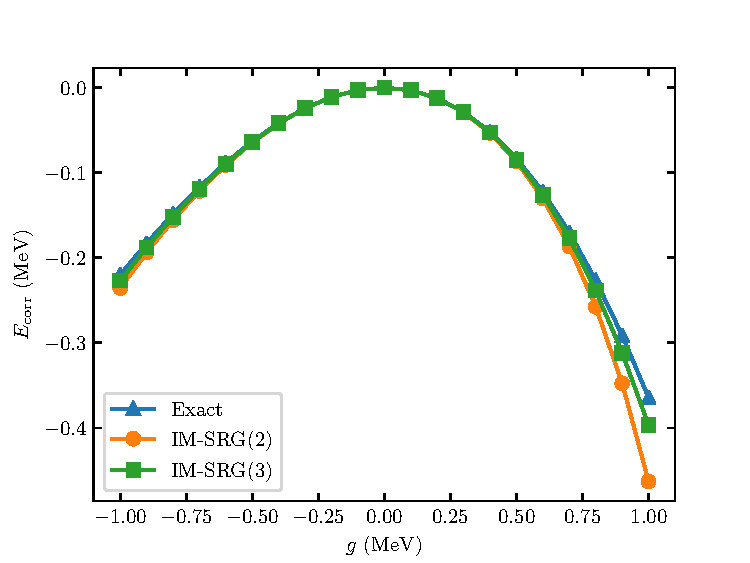
\includegraphics[width=0.9\textwidth]{proposal/doc/images/pairing_ham_imsrg3.pdf}
  \caption[
    The correlation energy $E_{\text{corr}}$ for the solution of the pairing Hamiltonian
    obtained via exact diagonalization,
    IM-SRG(2), and IM-SRG(3)
    for $-1 \le g \le 1$.
  ]{
    The correlation energy $E_{\text{corr}}$ for the solution of the pairing Hamiltonian
    obtained via exact diagonalization,
    IM-SRG(2), and IM-SRG(3)
    for $-1 \le g \le 1$.
    Exact diagonalization results obtained using code published with Ref.~\cite{Liet16lecnotesphysics}.
  }\label{fig:pairing_hamiltonian_fig}
\end{figure}

Thus, we are interested in the correlation energy obtained by the IM-SRG(2) and IM-SRG(3) solutions,
defined as
\begin{equation}
  E_{\text{corr}} = E(\infty) - E(0)\,.
\end{equation}
This is plotted in Fig.~\ref{fig:pairing_hamiltonian_fig} for $-1 \le g \le 1$.
We find generally good agreement between the IM-SRG correlation energy
and the exact correlation energy,
with the exception of the region for $0.5 \le g \le 1$.
Here, the IM-SRG(3) calculation improves upon the relatively large error in the IM-SRG(2)
correlation energy,
which in Ref.~\cite{Herg16imsrglecnotes}
was explained as being due to an overcounting in the fourth-order diagrams in MBPT
by a factor of 1/2 present in the IM-SRG(2) truncation.
It seems that this overcounting at fourth-order is lifted in the IM-SRG(3)
replaced by some overcounting at a higher MBPT order,
where the contributions are smaller in magnitude.
We note here that our results for IM-SRG(2) match exactly with those from Ref.~\cite{Herg16imsrglecnotes}.

\section{\texorpdfstring{${}^4\text{He}$}{Helium-4}}

The second system we consider here is ${}^4\text{He}$,
the lightest closed-shell nucleus.
Before we begin a discussion about the details of the system,
a few comments are in order.
The following calculation is restricted to a very small modelspace,
one insufficient to achieve converged results for observables.
This is because our implementation does not take advantage of the rotational invariance
of spherically symmetric systems,
that is, that the normal-ordered two- and three-body Hamiltonians
are diagonal in $J$ and $\mathcal{J}$
and independent of $M_{J}$ and $M_{\mathcal{J}}$.
The exploitation of the symmetries leads to so-called $J$-scheme IM-SRG flow equations.
The current results are a benchmark implementation for the IM-SRG(2)
that are compared against an existing IM-SRG(2) $J$-scheme implementation~\cite{Stro15imsrgcpp}.
This serves as an additional validation of our implementation
in addition to the results for the pairing Hamiltonian.
The current implementation will serve as a benchmark
against which we can compare our $J$-scheme IM-SRG(3) implementation,
which will be the focus of the next phase of this project.

As input into our calculation, we start with the intrinsic $A$-body Hamiltonian
with only an initial two-body interaction,
\begin{equation}
  H_{\text{int}} = T_{\text{int}} + \twobodyop{V}\,,
\end{equation}
with the intrinsic kinetic energy
\begin{align}
  T_{\text{int}} &= T - T_{\text{cm}} \\
                 &= \left(1 - \frac{1}{A}\right) \sum_{i} \frac{p_{i}^{2}}{2m}
                 - \frac{1}{A}\sum_{i<j}\frac{p_{i} \cdot p_{j}}{m}\,.
\end{align}
We note that the first term gives us our one-body Hamiltonian
and the second term contributes to the two-body Hamiltonian along with $\twobodyop{V}$~\cite{Herg09intrinsicham}.

We work in the single-particle harmonic-oscillator basis
at several different values of $\hbar \Omega$
(see Section~\ref{sec:sp_ho}),
with the single-particle states
\begin{equation}
  \ket{n_a (l_a s_a) j_a m_{j_a} t_a m_{t_a}} \equiv \ket{\alpha_a}\,,
\end{equation}
where $s_a=1/2$ and $t_a=1/2$.
A natural ordering of these states is according to their energy quantum number,
$e = 2  n + l$.
For the following calculation, we truncate the single-particle basis at $\emax=2$.
The resulting size of our single-particle basis is $N=40$.
As our reference state for ${}^4\text{He}$ we choose to fill the four $e=0$ HO states,
the most reasonable choice to target the ground state
without solving for and transforming to the Hartree-Fock basis.

\begin{figure}[t]
  \centering
  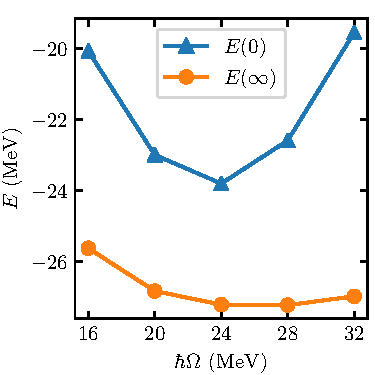
\includegraphics[width=0.45\textwidth]{proposal/doc/images/he4_imsrg2_energies.pdf}
  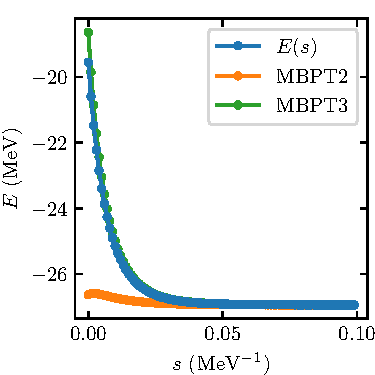
\includegraphics[width=0.45\textwidth]{proposal/doc/images/he4_imsrg2_flow.pdf}
  \caption[
    The left panel shows $E(0)$ and $E(\infty)$
    for an IM-SRG(2) calculation of ${}^4\text{He}$
    for $\hbar \Omega$ ranging from $16\mev$ to $32\mev$.
    The interaction used is the EM NN interaction
    with a regulator cutoff $\Lambda=500\mev$
    and SRG-evolved to $\lambda=1.8\invfm$.
    The right panel shows the flowing energy $E(s)$
    along with the energy with second- and third-order MBPT corrections included
    for $\hbar \Omega=32\mev$.
  ]{
    The left panel shows $E(0)$ and $E(\infty)$
    for an IM-SRG(2) calculation of ${}^4\text{He}$
    for $\hbar \Omega$ ranging from $16\mev$ to $32\mev$.
    The interaction used is the EM NN interaction
    with a regulator cutoff $\Lambda=500\mev$
    and SRG-evolved to $\lambda=1.8\invfm$~\cite{Ente03n3lonn}.
    The right panel shows the flowing energy $E(s)$
    along with the energy with second- and third-order MBPT corrections included
    for $\hbar \Omega=32\mev$.
  }\label{fig:imsrg2_he4_results}
\end{figure}

For $\twobodyop{V}$, we use the EM NN potential from Ref.~\cite{Ente03n3lonn} at N3LO
with a regulator cutoff at $\Lambda=500\mev$ and SRG-evolved to $\lambda=1.8\invfm$.
This potential has been shown to reproduce experimental binding energies
across the nuclear chart very well~\cite{Hebe20habi}.
The results from normal ordering our Hamiltonians at the different $\hbar \Omega$
with respect to our HO reference state
and evaluating the IM-SRG(2) evolution are shown
in the left panel of Fig.~\ref{fig:imsrg2_he4_results}.
We find that the unevolved energy $E(0)$,
that is, the energy expectation value of the reference state,
is already good to within 30\% of the exact result,
a consequence of the SRG-softened interaction we are using.
Still, the IM-SRG evolution absorbs up to $8\mev$ of correlation energy into the ground-state energy.
We also find that our implementation agrees with the implementation from Ref.~\cite{Stro15imsrgcpp}
to within $10^{-5}\mev$.

In the right panel of Fig.~\ref{fig:imsrg2_he4_results},
we show the flowing ground-state energy
as well as the ground-state energy with second- and third-order MBPT corrections.
We find that these corrections vanish as the correlations are absorbed into the ground-state energy,
indicating that we are achieving the desired decoupling.
We emphasize once again that these results are intended to be interpreted as validation
(for example, as a nuclear-like toy model)
and not as physically meaningful.
We consider the agreement between our implementation and that of Ref.~\cite{Stro15imsrgcpp}
to be \textit{a posteriori} evidence of the correctness of our implementation.



\chapter{Summary and outlook}\label{ch:summary}

In this thesis, we aim to study the ground-state properties of closed-shell nuclear systems in the IM-SRG(3).
As a first step in that direction, we have implemented a generic IM-SRG(2)/(3) solver,
which we applied at the IM-SRG(2) truncation level to the calculation of the ${}^4\text{He}$ ground-state energy
and at the IM-SRG(2) and IM-SRG(3) level to the pairing Hamiltonian.
At the IM-SRG(2) level, we found excellent agreement between our implementation
and existing IM-SRG(2) implementations and published results~\cite{Stro15imsrgcpp,Herg16imsrglecnotes}.
For the pairing Hamiltonian at the IM-SRG(3) level,
we found that the three-body truncation does reduce the discrepancy between IM-SRG(2) and the exact solution
in the region of large coupling.
This can be interpreted as evidence that the many-body expansion is behaving systematically,
a claim that we would also like to verify in nuclear systems.

In principle, the next step would be to calculate ${}^4\text{He}$
with the same Hamiltonian in the IM-SRG(3),
where one would expect the corrections due to the three-body truncation to be small.
With our $\emax=2$, this amounts to solving a system of approximately 4 billion coupled differential equations,
most of which are the flowing matrix elements of the three-body Hamiltonian $W$.
Of course, many of these matrix elements are not independent,
related to one another via antisymmetry or (anti-)Hermiticity,
and many should be exactly equal to 0,
such as those that are blocked by the Pauli exclusion principle.
By exploiting these symmetries, it may be possible to allow the current implementation
of IM-SRG(3) to also work for ${}^4\text{He}$.
This would offer the ability to look at many different metrics,
such as the flowing ground-state energy and the MBPT corrections,
when implementing a $J$-scheme IM-SRG(3) library.
Even if the performance is insufficient, a calculation can be run for a few integration steps
and the implementation of the fundamental commutators can be used
to benchmark the $J$-scheme implementation of the fundamental commutators.

Looking forward to the next phase of the project,
some key deliverables will be:
\begin{enumerate}
  \item{
    implementing a correct $J$-scheme IM-SRG(3) solver
    for use in nuclear many-body calculations
    using automatic recoupling tools~\cite{Tich20jcoupling};
  }
  \item tuning the performance of the solver to reach single-particle basis sizes large enough
    for observables to be reasonably converged;
  \item calculating the ground-state energies (and possibly other observables) for ${}^4\text{He}$
    and ${}^{16}\text{O}$ in the IM-SRG(3) and systematically studying the effects of the three-body truncation.
\end{enumerate}
It will be interesting to see if the improvement looks significantly different for different Hamiltonians
and if there are some well-reasoned physically-motivated ways to approximate the IM-SRG(3) well
that could be used to extend current large-scale IM-SRG(2) implementations.
Some options for such approximations might be
the inclusion of certain terms that dominate the IM-SRG(3) contributions
or the development of a way to include sparse approximate three-body operators
that provide the dominant IM-SRG(3) contributions.
With a robust implementation of our own,
we will be in an excellent position to systematically study these options and many more.



\begin{appendices}

% \include{proposal/doc/a01}

\end{appendices}

\backmatter{}

\bibliographystyle{unsrt} % use your favorite BIBTeX style
% \nocite{*} % To display all refs, even uncited refs (useful when editting)
\bibliography{sources}

\end{document}

